% In this file you should put the actual content of the blueprint.
% It will be used both by the web and the print version.
% It should *not* include the \begin{document}
%
% If you want to split the blueprint content into several files then
% the current file can be a simple sequence of \input. Otherwise It
% can start with a \section or \chapter for instance.

% TODO: CONVERT ALL SPELLINGS TO AMERICAN! DON'T STANDARDISE: STANDARDIZE!

\begin{abstract}
  This blueprint consists of an adaptation of Maryna Viazovska's Fields Medal-winning paper proving that no packing of unit balls in Euclidean space $\R^8$ has density greater than that of the $E_8$-lattice packing.
  \ifplastex
  % web
  You can view the contents of the current version of this page in PDF form \href{https://thefundamentaltheor3m.github.io/Sphere-Packing-Lean/blueprint.pdf}{here}.
  \else
  % print
  We recommend that you look at \href{https://thefundamentaltheor3m.github.io/Sphere-Packing-Lean/blueprint/index.html}{this webpage} for the latest version.
  \fi \\

  This formalisation project was kickstarted at EPFL by Maryna Viazovska and Sidharth Hariharan, and the contents of this blueprint were originally written by Maryna Viazovska on the suggestion of Kevin Buzzard. It is being updated and restructured by those involved in the formalisation effort, namely, Sidharth Hariharan, Gareth Ma, Seewoo Lee and Christopher Birkbeck. Those involved in the effort express their sincere gratitude to Kevin Buzzard, Utensil Song, Bhavik Mehta, Patrick Massot, Yaël Dillies, and everyone in the Lean Community for their support.
  \end{abstract}

\tableofcontents

\pagebreak
% \section{draft}
%
% We denote the open ball centered at $c \in \R^n$ with radius $r$ by $\mathcal{B}(c; r) \coloneqq \{x \in \R^n : \|x - c\| < r\}$. By abuse of notation, we also write $\mathcal{B}(\mathcal{P}; r) \coloneqq \bigcup_{c \in \mathcal{P}} \mathcal{B}(c; r)$. For us, the balls will always be disjoint.
%
% \begin{definition}
%   Let $\mathcal{P} \subseteq \R^d$ be a set of vectors such that $\forall x \neq y \in \mathcal{P}, \|x - y\| \geq 2$. We define the \emph{density} of $\mathcal{P}$ to be
%
%   \[
%     \Delta_{\mathcal{P}} \coloneqq \lim_{R \to \infty} \frac{\mathrm{Vol}(\mathcal{B}(\mathcal{P}; 1) \cap \mathcal{B}(0; R))}{\mathrm{Vol}(\mathcal{B}(0; R))}
%   \]
% \end{definition}
%
% \begin{definition}
%   Let $\Lambda \subseteq \R^d$ be a $\Z$-lattice, and suppose further that the $\mathcal{P}$ above also satisfy $\forall g \in \Lambda, \forall v \in \mathcal{P}, g + v \in \mathcal{P}$. We define the \emph{periodic density} of $\mathcal{P}$ to be
%
%   \[
%     \Delta_{\mathcal{P}, \Lambda}^{periodic} \coloneqq \frac{\mathrm{Vol}(\mathcal{B}(\mathcal{P}; 1) \cap \Lambda)}{\mathrm{Vol}(\Lambda)}
%   \]
% \end{definition}
%
% \begin{theorem}
%   \[
%     \Delta_{\mathcal{P}} = \Delta_{\mathcal{P}, \Lambda}^{periodic}
%   \]
% \end{theorem}
% \begin{proof}
%   \todo{Help.}
% \end{proof}
%
\section{Sphere packings}\label{sec:sphere-packings}
\subsection{Sphere packings}

The sphere packing constant measures which portion of $d$_dimensional Euclidean space can be covered by non_overlapping unit balls. More precisely, let $\R^d$ be the Euclidean vector space equipped with distance $\|\cdot\|$ and Lebesgue measure $\mathrm{Vol}(\cdot)$. For $x\in\R^d$ and $r\in\R_{>0}$ we denote by $B_d(x,r)$ the ball in $\R^d$ with center $x$ and radius $r$. There are several types of sphere packings, which are determined by imposing certain conditions on the set of centres of the spheres involved in the packing. Therefore, we begin by defining those conditions on the centres of the spheres.

Below, $c$ is any real number (the scaling factor), usually with constraints such as $c > 0$ or $c \neq 0$.

\begin{definition}\label{SpherePacking.SpherePackingCentres}\lean{SpherePacking.SpherePackingCentres}\leanok
  We say that $X \subseteq \R^d$ is a set of \emph{sphere packing centres with separation $r$} if $X$ is discrete and $\|x _ y\| \geq r$ for all $x \neq y\in X$.
\end{definition}

\begin{definition}\label{SpherePacking.LatticePackingCentres}\lean{SpherePacking.LatticePackingCentres}\uses{SpherePacking.SpherePackingCentres}\leanok
  We say that $X \subseteq \R^d$ is a set of \emph{lattice packing centres with separation $r$} if $X$ is both a set of sphere packing centres with separation $r$ and a lattice in $\R^d$.
\end{definition}

\begin{definition}\label{SpherePacking.Packing_of_Centres}\lean{SpherePacking.Packing_of_Centres}\leanok  % Do we want to replace the notation \mathcal{P} with \mathcal{P}_X or \mathcal{P}(X)?
  Let $X\subset \R^d$ be a set of sphere packing centres of separation $r$. Then, the set $$\mathcal{P} = \bigcup_{x \in X} B_d\left(x, \frac{r}{2}\right)$$ of unit balls centred at points in $X$ is the corresponding \emph{sphere packing}.
\end{definition}

\begin{remark}
  If $X$ is a set of lattice/periodic packing centres (see \cref{SpherePacking.LatticePackingCentres,SpherePacking.PeriodicPackingCentres}), then the corresponding sphere packing $\mathcal{P}$ is called a \emph{lattice/periodic packing}.
\end{remark}

\begin{definition}\label{SpherePacking.FiniteDensity}\lean{SpherePacking.FiniteDensity}\uses{SpherePacking.Packing_of_Centres}\leanok
  The \emph{finite density} of a packing $\mathcal{P}$ is defined as
$$\Delta_{\mathcal{P}}(R):=\frac{\mathrm{Vol}(\mathcal{P}\cap B_d(0,R))}{\mathrm{Vol}(B_d(0,R))},\quad R>0.$$
\end{definition}

\begin{definition}\label{SpherePacking.Density}\lean{SpherePacking.Density}\uses{SpherePacking.Packing_of_Centres, SpherePacking.FiniteDensity}\leanok
  We define the \emph{density} of a packing $\mathcal{P}$ as the limit supremum
$$\Delta_{\mathcal{P}}:=\limsup\limits_{R\to\infty}\Delta_{\mathcal{P}}(R). $$
\end{definition}

\begin{definition}\label{SpherePacking.Constant}\lean{SpherePacking.Constant}\uses{SpherePacking.Packing_of_Centres, SpherePacking.Density}\leanok
  The sphere packing problem is to compute the \emph{sphere packing constant}, defined as supremum of packing densities over all possible packing
$$\Delta_d:=\sup\limits_{\substack{\mathcal{P}\subset\R^d\\ \scriptscriptstyle\mathrm{sphere}\;\mathrm{packing}}}\Delta_{\mathcal{P}}.$$
\end{definition}

\subsection{Scaling Sphere Packings}

Given that the problem involves the \emph{arrangement} of balls in space, it is intuitive not to worry about the radius of the balls (so long as they are all equal to each other). However, Definition~\ref{SpherePacking.balls} involves a choice of separation radius. In principle, we would want two sphere packing configurations that differ only in separation radii to `encode the same information'. In this brief subsection, we will describe how to change the separation radius of a sphere packing by \emph{scaling} the packing by a positive real number and prove that this does not affect its density. This will give us the freedom to choose any separation radius we like when attempting to define the optimal sphere packing in $\R^d$.

\begin{definition}\label{SpherePacking.scale}\lean{SpherePacking.scale}\uses{SpherePacking}\leanok
  Given a sphere packing $\Pa(X)$ with separation radius $r$, we defined the \emph{scaled packing} with respect to a real number $c > 0$ to be the packing $\Pa(cX)$, where $cX = \setof{cx \in V}{x \in X}$ has separation radius $cr$.
\end{definition}

\begin{lemma}\label{SpherePacking.scale_finiteDensity}\lean{SpherePacking.scale_finiteDensity}\uses{SpherePacking.finiteDensity, SpherePacking.scale}\leanok
  Let $\Pa(X)$ be a sphere packing and $c$ a positive real number. Then, for all $R > 0$,
  \[
    \Delta_{\Pa(cX)}(cR) = \Delta_{\Pa(X)}(R).
  \]
\end{lemma}
\begin{proof}
  The proof follows by direct computation:
  \[
    \Delta_{\Pa(cX)}(cR) = \frac{\Vol{\Pa(cX) \cap B_d(0, cR)}}{\Vol{B_d(0, cR)}} = \frac{c^d \cdot \Vol{\Pa(X) \cap B_d(0, R)}}{c^d \cdot \Vol{B_d(0, R)}}
    % = \frac{\Vol{\Pa(X) \cap B_d(0, R)}}{\Vol{B_d(0, R)}}
    = \Delta_{\Pa(X)}(R)
  \]
  where the second equality follows from applying the fact that scaling a (measurable) set by a factor of $c$ scales its volume by a factor of $c^d$ to the fact that $\Pa(cX) \cap B_d(0, cR) = c \cdot (\Pa(X) \cap B_d(0, cR))$.
\end{proof}

\begin{lemma}\label{SpherePacking.scale_density}\lean{SpherePacking.scale_density}\uses{SpherePacking.scale}\leanok
  Let $\Pa(X)$ be a sphere packing and $c$ a positive real number. Then, the density of the scaled packing $\Pa(cX)$ is equal to the density of the original packing $\Pa(X)$.
\end{lemma}
\begin{proof}\uses{SpherePacking.scale_finiteDensity}
  One can show, using relatively unsophisticated real analysis, that
  \[
    \limsup_{R \to \infty} \Delta_{\Pa(cX)}(R) = \limsup_{cR \to \infty} \Delta_{\Pa(cX)}(cR)
  \]
  Lemma~\ref{SpherePacking.scale_finiteDensity} tells us that $\Delta_{\Pa(cX)}(cR) = \Delta_{\Pa(X)}(R)$ for every $R > 0$. Therefore,
  \[
    \limsup_{cR \to \infty} \Delta_{\Pa(cX)}(cR) = \limsup_{cR \to \infty} \Delta_{\Pa(X)}(R) = \limsup_{R \to \infty} \Delta_{\Pa(X)}(R)
  \]
  where the second equality is the result of a similar change of variables to the one done above.
\end{proof}

Therefore, as expected, we do not need to worry about the separation radius when constructing sphere packings. This will be useful when we attempt to construct the optimal sphere packing in $\R^8$---and even more so when attempting to \emph{formalise} this construction---because the underlying structure of the packing is given by a set known as the $E_8$ lattice, which has separation radius $\sqrt{2}$.

We can also use Lemma~\ref{SpherePacking.scale_density} to simplify the computation of the sphere packing constant by taking the supremum not over \emph{all} sphere packings but only over those with density $1$.

\begin{lemma}\label{SpherePacking.constant_eq_constant_normalized}\lean{SpherePacking.constant_eq_constant_normalized}\uses{SpherePackingConstant, SpherePacking.density}\leanok
  \[
    \Delta_d = \sup\limits_{\substack{\Pa \subset \R^d \\ \text{sphere packing} \\ \text{sep.~rad.} = 1}} \Delta_{\Pa}
  \]
\end{lemma}
\begin{proof}\uses{SpherePacking.scale_density}
  That the supremum over packings of unit density is at most the sphere packing constant is obvious. For the reverse inequality, let $\Pa(X)$ be any sphere packing with separation radius $r$. We know, from Lemma~\ref{SpherePacking.scale_density}, that the density of $\Pa(X)$ is equal to that of the scaled packing $\Pa\!\left(\frac{X}{r}\right)$. Since the scaled packing has separation radius $1$, its density is naturally at most the supremum over all packings of unit density, meaning that the same is true of $\Pa(X)$.
\end{proof}

\subsection{Lattices and Periodic packings}

\begin{definition}\label{EuclideanLattice.isLattice}\lean{EuclideanLattice.isLattice}\leanok
  % A lattice in the Euclidean space $\R^d$ is a discrete, co-compact, abelian subgroup.
  We say that an additive subgroup $\Lambda \leq \R^d$ is a \emph{lattice} if it is discrete and its $\R$-span contains all the elements of $\R^d$.
\end{definition}


\begin{definition}\label{SpherePacking.PeriodicPackingCentres}\lean{SpherePacking.PeriodicPackingCentres}\uses{SpherePacking.SpherePackingCentres, EuclideanLattice.isLattice}\leanok
  We say that $X \subseteq \R^d$ is a set of \emph{periodic packing centres} if $X$ is a set of sphere packing centres and there exists a lattice $\Lambda \subset \R^d$ such that for any $x \in X$ and $y \in \Lambda$, their sum $x + y$ lies in $X$.
\end{definition}

\begin{lemma}\label{SpherePacking.Density of periodic packing}\notready
  If $X \subseteq \R^d$ is a set of sphere packing centres that is periodic with respect to some lattice $\Lambda$, then the density of the corresponding (periodic) sphere packing is given by
  $$ \frac{\lvert {X/\Lambda} \rvert}{\mathrm{Vol}(\R^d / \Lambda)} \cdot \mathrm{Vol}(B_d(0,1))$$
  where the quotients in the numerator and denominator correspond to the orbits of the action by translation of $\Lambda$ on $X$ and $\R^d$ respectively.
\end{lemma}
\begin{remark}
  This can be thought of as the ``volume of spheres per fundamental domain": the number of spheres per fundamental domain is $\lvert {X/\Lambda} \rvert$, and the volume of each sphere is $\mathrm{Vol}(B_d(0,1))$.
\end{remark}

\begin{definition}\label{def-Periodic-sphere-packing-constant}\uses{SpherePacking.Density, SpherePacking.PeriodicPackingCentres}\notready
    The periodic sphere packing constant is defined to be
    $$ \Delta_{d}^{\text{periodic}} := \sup_{\substack{P \subset \R^d \\ \text{periodic packing}}} \Delta_P$$
\end{definition}

\begin{theorem}\label{periodic-packing-optimal}\uses{SpherePacking.Density, def-Periodic-sphere-packing-constant}\notready
    For all $d$, the periodic sphere packing constant in $\R^d$ is equal to the sphere packing constant in $\R^d$.
\end{theorem}
\begin{proof}
  \todo{State this in Lean (ready).}
  \todo{Fill in proof here (see~\cite[Appendix A]{ElkiesCohn}}
\end{proof}

In other words, it suffices to compute and optimise the periodic sphere packing constant.

\subsection{Density of periodic packings}

In this subsection, we build up results about the density of periodic packings. In particular, the density of a periodic packing, defined as the limit of the periodic packing intersected with a growing ball centered at the origin, is equal to the density within any fundamental region of the period lattice.

% \todo{Actually add results here.}

\subsection{Main Result}

With the terminologies above, we can state the main theorem of this project.

\begin{theorem}\label{Main}\lean{Main}\uses{E8_Scaled_Lattice, SpherePacking.Constant, SpherePacking.Density}
  All \emph{periodic} packing $\mathcal{P} \subseteq \R^8$ has density satisfying $\Delta_{\mathcal{P}} \leq \Delta_{E_8}$, the density of the $E_8$ sphere packing (see Definition~\ref{E8_Packing}).
\end{theorem}
\begin{proof}
  We will prove this theorem over the course of this blueprint.
  % TODO: Add a \ref to the actual proof at the end of this blueprint, I guess.
\end{proof}

\begin{corollary}\label{Main'}\lean{Main'}\uses{Main, periodic_packing_optimal}
  All packing $\mathcal{P} \subseteq \R^8$ has density satisfying $\Delta_{\mathcal{P}} \leq \Delta_{E_8}$.
\end{corollary}
\begin{proof}
  This is a direct consequence of Theorem~\ref{periodic_packing_optimal} and Theorem~\ref{Main}.
\end{proof}

\begin{corollary}\label{Main''}\uses{Main'}
  $\Delta_8 = \Delta_{E_8}$.
\end{corollary}
\begin{proof}
  By definition, $\Delta_{E_8} \leq \Delta_8$, while Corollary~\ref{Main'} shows $\Delta_8 = \sup_{\mathrm{packing} \, \mathcal{P}} \leq \Delta_{E_8}$, and the result follows.
\end{proof}


\pagebreak
\section{Density of packings}\label{sec:packings-density}

\subsection{Bounds on Finite Density of Packing}

We first collect all the results we will prove here, then prove them separately below. We do this because some are proven already! Let $X \subseteq \R^d$ be a set of sphere packing centers with separation $r$.

\begin{theorem}\label{finite-density-bounds}\uses{}\leanok
  We have the following theorem relating the finite density and the number of lattice points in a ball:

  \[
    \left|X \cap \mathcal{B}_d\left(R - \frac{r}{2}\right)\right| \cdot \frac{\mathrm{Vol}\left(\mathcal{B}_d\left(\frac{r}{2}\right)\right)}{\mathrm{Vol}(\mathcal{B}_d(R))}
    \leq \Delta_{\mathcal{P}}(R)
    \leq \left|X \cap \mathcal{B}_d\left(R + \frac{r}{2}\right)\right| \cdot \frac{\mathrm{Vol}\left(\mathcal{B}_d\left(\frac{r}{2}\right)\right)}{\mathrm{Vol}(\mathcal{B}_d(R))}
  \]
\end{theorem}
\begin{proof}
  Proven by Gareth already. The high level idea is to prove that $\mathcal{P} \cap \mathcal{B}_d(R) = \left(\bigcup_{x \in X} \mathcal{B}_d\left(x, \frac{r}{2}\right)\right) \subseteq \bigcup_{x \in X \cap \mathcal{B}_d\left(R + \frac{r}{2}\right)} \mathcal{B}_d\left(x, \frac{r}{2}\right)$, and a similar inequality for the upper bound. The rest follows by rearranging and usign the fact that the balls are pairwise disjoint.
\end{proof}

Suppose further that $X$ is a periodic packing w.r.t. the lattice $\Lambda \subseteq \R^d$. Let $\mathcal{D}$ be a fundamental region of $\Lambda$, say the parallelopiped defined in the proof of \cref{exists-bounded-fd}, and let $L$ be the bound on the norm of vectors in $\mathcal{D}$ (see \cref{exists-bounded-fd}).

\begin{theorem}\label{lattice-points-bounds}\uses{lattice-points-bounds-proof}
  For real numbers $R > L$, we have the following inequality relating the number of lattice points from $\Lambda$ in a ball with the volume of the ball and the fundamental region $\mathcal{D}$:

  \[
    \frac{\mathrm{Vol}(\mathcal{B}_d(R - L))}{\mathrm{Vol}(\mathcal{D})}
    \leq \left|\Lambda \cap \mathcal{B}_d(R)\right|
    \leq \frac{\mathrm{Vol}(\mathcal{B}_d(R + L))}{\mathrm{Vol}(\mathcal{D})}
  \]
\end{theorem}

The proof can be found at \cref{lattice-points-bounds-proof}.

\begin{theorem}\label{periodic-points-bounds}\uses{periodic-points-bounds-proof}
  For real numbers $R > L$, we have the following inequality relating the number of points from $X$ (periodic w.r.t. $\Lambda$) in a ball with the number of points from $\Lambda$:

  \[
    \left|\Lambda \cap \mathcal{B}_d(R - L)\right|\left|X / \Lambda\right|
    \leq \left|X \cap \mathcal{B}_d(R)\right|
    \leq \left|\Lambda \cap \mathcal{B}_d(R + L)\right|\left|X / \Lambda\right|
  \]
\end{theorem}

\todo{Link the proof}

Finally, when we combine the inequalities above, we need one additional computational lemma.

\begin{lemma}\label{volume-ball-ratio}
  For any constant $C > 0$, we have

  \[
    \lim_{R \to \infty} \frac{\mathrm{Vol}(\mathcal{B}_d(R))}{\mathrm{Vol}(\mathcal{B}_d(R + C))} = 1
  \]
\end{lemma}
\begin{proof}
  Write out the formula for volume of a ball and simplify. More specifically, we have $\mathrm{Vol}(\mathcal{B}_d(R)) = R^d \pi^{d / 2} / \Gamma\left(\frac{d}{2} + 1\right)$, so $\mathrm{Vol}(\mathcal{B}_d(R)) / \mathrm{Vol}(\mathcal{B}_d(R + C)) = R^d / (R + C)^d = \left(1 - \frac{1}{R + C}\right)^d = 1$.
\end{proof}

% \begin{lemma}\label{volume-balls-ratio}\uses{}
%   We have
%
%   \[
%     \lim_{R \to \infty} \frac{
%   \]
% \end{lemma}

% \begin{theorem}\label{}


\pagebreak
\section{The $E_8$ lattice}
\subsection{Definitions of $E_8$ lattice}

There are several equivalent definitions of the $E_8$ lattice. Below, we formalise two of them, and prove they are equivalent.

\begin{definition}{($E_8$-lattice, Definition 1)}\label{E8-Set}\lean{E8.E8_Set}\leanok
  We define the \emph{$E_8$-lattice} (as a subset of $\R^8$) to be
$$\Lambda_8=\{(x_i)\in\Z^8\cup(\Z+\textstyle\frac12\displaystyle )^8|\;\sum_{i=1}^8x_i\equiv 0\;(\mathrm{mod\;2})\}.$$
\end{definition}

\begin{definition}{($E_8$-lattice, Definition 2)}\label{E8-Matrix}\lean{E8.E8_Matrix}\leanok
  We define the \emph{$E_8$ basis vectors} to be the set of vectors
  \[ \B_8 =
  \left\{
    \begin{bmatrix}
      1 \\ -1 \\ 0 \\ 0 \\ 0 \\ 0 \\ 0 \\ 0
    \end{bmatrix},
    \begin{bmatrix}
      0 \\ 1 \\ -1 \\ 0 \\ 0 \\ 0 \\ 0 \\ 0
    \end{bmatrix},
    \begin{bmatrix}
      0 \\ 0 \\ 1 \\ -1 \\ 0 \\ 0 \\ 0 \\ 0
    \end{bmatrix},
    \begin{bmatrix}
      0 \\ 0 \\ 0 \\ 1 \\ -1 \\ 0 \\ 0 \\ 0
    \end{bmatrix},
    \begin{bmatrix}
      0 \\ 0 \\ 0 \\ 0 \\ 1 \\ -1 \\ 0 \\ 0
    \end{bmatrix},
    \begin{bmatrix}
      0 \\ 0 \\ 0 \\ 0 \\ 0 \\ 1 \\ 1 \\ 0
    \end{bmatrix},
    \begin{bmatrix}
      -1/2 \\ -1/2 \\ -1/2 \\ -1/2 \\ -1/2 \\ -1/2 \\ -1/2 \\ -1/2
    \end{bmatrix},
    \begin{bmatrix}
      0 \\ 0 \\ 0 \\ 0 \\ 0 \\ 1 \\ -1 \\ 0
    \end{bmatrix}
  \right\}
  \]
\end{definition}

% Forward direction hasn't been proven yet
\begin{theorem}\label{E8-defs-equivalent}\lean{E8.E8_Set_eq_span}\uses{E8-Set, E8-Matrix}\leanok
  The two definitions above coincide, i.e. $\Lambda_8 = \mathrm{span}_{\Z}(\B_8)$.
\end{theorem}
\begin{proof}
  We prove each side contains the other side.

  For a vector $\vec{v} \in \Lambda_8 \subseteq \R^8$, we have $\sum_i \vec{v}_i \equiv 0 \pmod{2}$ and $\vec{v}_i$ being either all integers or all half-integers. After some modulo arithmetic, it can be seen that $\B_8^{-1}\vec{v}$ as integer coordinates (i.e. it is congruent to $0$ modulo $1$). Hence, $\vec{v} \in \mathrm{span}_{\Z}(\B_8)$.

  For the opposite direction, we write the vector as $\vec{v} = \sum_i c_i\B_8^i \in \mathrm{span}_{\Z}(\B_8)$ with $c_i$ being integers and $\B_8^i$ being the $i$-th basis vector. Expanding the definition then gives $\vec{v} = \left(c_1 - \frac{1}{2}c_7, -c_1 + c_2 - \frac{1}{2}c_7, \cdots, -\frac{1}{2}c_7\right)$. Again, after some modulo arithmetic, it can be seen that $\sum_i \vec{v}_i$ is indeed $0$ modulo $2$ and are all either integers and half-integers, concluding the proof.

  (Note: this proof doesn't depend on that $\B_8$ is linearly independent.)
\end{proof}

\subsection{Basic Properties of $E_8$ lattice}

In this section, we establish basic properties of the $E_8$ lattice and the $\B_8$ vectors.

\begin{lemma}\label{E8-is-basis}\lean{E8.E8_is_basis}\uses{E8-Matrix}\leanok
  $B_8$ is a $\R$-basis of $\R^8$.
\end{lemma}
\begin{proof}
  It suffices to prove that $\B_8 \in \mathrm{GL}_8(\R)$. We prove this by explicitly defining the inverse matrix $\B_8^{-1}$ and proving $\B_8 \B_8^{-1} = I_8$, which implies that $\det(\B_8)$ is nonzero. See the Lean code for more details.,
\end{proof}

\begin{lemma}\label{E8-Lattice}\lean{E8.E8_Lattice}\uses{E8-Set, E8-defs-equivalent}\leanok
  $\Lambda_8$ is an additive subgroup of $\R^8$.
\end{lemma}
\begin{proof}\leanok
  Trivially follows from that $\Lambda_8 \subseteq \R^8$ is the $\Z$-span of $\B_8$ and hence an additive group.
\end{proof}

\begin{lemma}\label{E8-vector-norms}\lean{E8.E8_norm_eq_sqrt_even}\uses{E8-defs-equivalent}\leanok
  All vectors in $\Lambda_8$ have norm of the form $\sqrt{2n}$, where $n$ is a nonnegative inteeger.
\end{lemma}
\begin{proof}
  Writing $\vec{v} = \sum_i c_i\B_8^i$, we have $\|v\|^2 = \sum_i \sum_j c_ic_j (\B_8^i \cdot \B_8^j)$. Computing all $64$ pairs of dot products and simplifying, we get a massive term that is a quadratic form in $c_i$ with even integer coefficients, concluding the proof.
\end{proof}

\begin{lemma}\label{instDiscreteE8Lattice}\lean{E8.instDiscreteE8Lattice}\uses{E8-vector-norms}\leanok
  $c\Lambda_8$ is discrete, i.e. that the subspace topology induced by its inclusion into $\R^8$ is the discrete topology.
\end{lemma}
\begin{proof}
  Since $\Lambda_8$ is a topological group and $+$ is continuous, it suffices to prove that $\{0\}$ is open in $\Lambda_8$. This follows from the fact that there is an open ball $\B(\sqrt{2}) \subseteq \R^8$ around it containing no other lattice points, since the shortest nonzero vector has norm $\sqrt{2}$.
\end{proof}

\begin{lemma}\label{instLatticeE8}\lean{E8.instIsZLatticeE8Lattice}\uses{instDiscreteE8Lattice, E8-is-basis}\leanok
  $c\Lambda_8$ is a $\Z$-lattice, i.e. it is discrete and spans $\R^8$ over $\R$.
\end{lemma}
\begin{proof}
  The first part is by \cref{instDiscreteE8Lattice}, and the second part follows from that $\B_8$ is a basis (\cref{E8-is-basis}) and hence linearly independent over $\R$.
\end{proof}

\todo{Prove $E_8$ is unimodular.}
\todo{Prove $E_8$ is positive-definite.}

\subsection{The $E_8$ sphere packing}

\begin{definition}\label{E8Packing}\lean{E8.E8Packing}\uses{E8-Lattice,E8-vector-norms}\leanok
  The \emph{$E_8$ sphere packing} is the (periodic) sphere packing with separation $\sqrt{2}$, whose set of centres is $\Lambda_8$.
\end{definition}

\begin{lemma}\label{E8Packing-covol}\lean{E8.E8_Basis_volume}\uses{E8Packing}
  $\Vol{\Lambda_8} = \mathrm{Covol}(\R^8 / \Lambda_8) = 1$.
\end{lemma}
\begin{proof}
  \todo{In theory this should follow directly from $\det(\Lambda_8) = 1$, but Lean hates me and \texttt{EuclideanSpace} is being annoying.}
\end{proof}

\begin{theorem}\label{E8Packing-density}\uses{theorem:psp-density,E8Packing-covol}\lean{E8.E8Packing_density}\leanok
  We have $\Delta_{\mathcal{P}(E_8)} = \frac{\pi^4}{384}$.
\end{theorem}
\begin{proof}\leanok
  By \cref{theorem:psp-density}, we have $\Delta_{\mathcal{P}(E_8)} = |E_8 / E_8| \cdot \frac{\Vol{\mathcal{B}_8(\sqrt{2} / 2)}}{\mathrm{Covol}(E_8)} = \frac{\pi^4}{384}$, where the last equality follows from \cref{E8Packing-covol} and the formula for volume of a ball: $\Vol{\mathcal{B}_d(R)} = R^d \pi^{d / 2} / \Gamma\left(\frac{d}{2} + 1\right)$.
\end{proof}


\pagebreak
\section{Facts from Fourier analysis}  % Specialise everything here from Mathlib
Recall the definition of a Fourier transform.

\begin{definition}\label{def:Fourier-Transform}\lean{Real.fourierIntegral}\leanok
  The Fourier transform of an $L^1$-function $f:\R^d\to\C$ is defined as

  \[
    \mathcal{F}(f)(y) = \widehat{f}(y) := \int_{\R^d} f(x)e^{-2\pi i \langle x, y \rangle} \,\mathrm{d}x, \quad y \in \R^d
  \]

  where $\langle x, y \rangle = \frac12\|x\|^2 + \frac12\|y\|^2 - \frac12\|x - y\|^2$ is the standard scalar product in $\R^d$.
\end{definition}

The following computational result will be of use later on.

\begin{lemma}\label{lemma:Gaussian-Fourier}\uses{def:Fourier-Transform}
  \begin{equation}
    \mathcal{F}(e^{\pi i \|x\|^2 z})(y) = z^{-4}\,e^{\pi i \|y\|^2 \,(\frac{-1}{z}) }.
  \end{equation}
\end{lemma}
\begin{proof}
  \todo{Fill in proof.}
\end{proof}

Of great interest to us will be a specific family of functions, known as Schwartz Functions. The Fourier transform behaves particularly well when acting on Schwartz functions. We elaborate in the following subsections.

\subsection{On Schwartz Functions}

\begin{definition}\label{def:Schwartz-Space}\lean{SchwartzMap}\leanok
A $C^\infty$~function $f:\R^d\to\C$ is called a \emph{Schwartz function} if it decays to zero as $\|x\|\to\infty$ faster then any inverse power of $\|x\|$, and the same holds for all partial derivatives of $f$, ie, if for all $k, n \in \N$, there exists a constant $C \in \R$ such that for all $x \in \R^d$, $\norm{x}^k \cdot \norm{f^{(n)}(x)} \leq C$, where $f^{(n)}$ denotes the $n$-th derivative of $f$ considered along with the appropriate operator norm. The set of all Schwartz functions from $\R^d$ to $\C$ is called the \emph{Schwartz space}. It is an $\R$-vector space.
\end{definition}

\begin{lemma}\label{lemma:Fourier-transform-is-automorphism}\lean{SchwartzMap.fourierTransformCLM}\uses{def:Fourier-Transform, def:Schwartz-Space}\leanok
  The Fourier transform is a continuous, linear automorphism of the space of Schwartz functions.
\end{lemma}
\begin{proof}\leanok
  We do not elaborate here as the result already exists in Mathlib. We do, however, mention that the Lean implementation \emph{defines} a continuous linear equivalence on the Schwartz space \emph{using} the Fourier transform (see \verb|SchwartzMap.fourierTransformCLM|). The `proof' that for any Schwartz function $f$, its Fourier transform and its image under this continuous linear equivalence are, indeed, the same $\R^d \to \R$ function, is stated in Mathlib solely for the purpose of \verb|rw| and \verb|simp| tactics, and is proven simply by \verb|rfl|.
\end{proof}

% Consider adding an example for expository effect (really not necessary, would be nice if time permits though)
Another reason we are interested in Schwartz Functions is that they behave well under infinite sums. This will be useful to us when proving the Cohn-Elkies linear programming bound.

\subsection{On the Summability of Schwartz Functions}

We begin by stating a general summability result over specific subsets of $\R^d$.

\begin{lemma}
  Let $X \subset \R^d$ be a set of sphere packing centres of separation $1$ that is periodic with some lattice $\Lambda \subset \R^d$. Then, there exists $k \in \N$ sufficiently large such that
  \[
    \sum_{x \in X} \frac{1}{\norm{x}^{k}} < \infty.
  \]
\end{lemma}
\begin{proof}
  First, note that it does not matter how we number the (countably many) elements of the discrete set $X$: if we prove absolute convergence for one numbering, we prove absolute convergence for \emph{any} numbering. The idea will be to bound the sequence of partial sums by considering the volumes of concentric $d$-spheres of the appropriate radii (or scaled versions of a $0$-centred fundamental domain).

  \todo{Finish!}

  % Number the elements of $X$ such that $\norm{x_1} \leq \norm{x_2} \leq \ldots$, and for all $R \in \N$, let $N_R$ be the largest index such that $\norm{x_{N_R}} \leq R$ (which exists because there can only be finitely many elements of $X$ in any ball of radius $R$). Define $S_R := \sum_{j=1}^{N_R} \norm{x_j}^{-k}$. If we can show that $S_R$ is a Cauchy sequence, we can show that $S_R$ (and therefore, $\sum_{j=1}^{\infty} \norm{x_j}^{-k}$) is convergent.

  % Fix $\eps > 0$. We need to find an $R \in \N$ such that for all $R < R_1 < R_2 \in \N$, $S_{R_2} - S_{R_1} < \eps$. We have that
  % \[
  %   0 \leq \sum_{j=N_{R_1}}^{N_{R_2}} \frac{1}{\norm{x_j}^k} \leq \frac{\Vol{\B_d(0, R_2)} - \Vol{B_d(0, R_1)}}{R_1^k} \leq \frac{c R_2^{d}}{R_1^k}
  % \]
  % for all $R > 1$. Then, for $k = d + 1$ (similarly for any $k > d$), we have some $c$ such that
  % \[
  %   0 \leq S_R \leq \frac{c}{R} \xrightarrow{R \to \infty} 0
  % \]
\end{proof}

The decaying property of Schwartz functions means that they can be compared to the absolutely convergent power series above.

\begin{lemma}
  Let $f : \R^d \to \C$ be a Schwartz function and let $X \subset \R^d$ be periodic with respect to some lattice $\Lambda \subset \R^d$. Then,
  \[
    \sum_{x \in X} |f(x)| < \infty.
  \]
\end{lemma}
\begin{proof}
  Without loss of generality, assume that $0 \notin X$: if $0 \in X$, then we can add the $f(0)$ term to the sum over nonzero elements of $X$, which, if the sum over the nonzero elements converges absolutely, will be equal to the sum over all of $X$. Now, we know that for all $k \in \N$, there exists some constant $C$ such that $|f(x)| \leq C\norm{x}^{-k}$ for all $x \in \R^d$. Choosing $k$ to be sufficiently large, we see that
  \[
    \sum_{x \in X} |f(x)| \leq \sum_{x \in X} \frac{C}{\norm{x}^{k}} = C \sum_{x \in X} \frac{1}{\norm{x}^k} < \infty.
  \]
\end{proof}

We end with a crucial result on Schwartz functions, the statement of which only makes sense because of the above result.
% Should probably include something about multiplying a Schwartz function by a negative exponential, either saying that the result is Schwartz (??) or by saying that it is summable. Both would be enough to make the RHS of the sum below converge absolutely.
\begin{theorem}[Poisson summation formula]\label{thm:Poisson-summation-formula}\uses{def:Fourier-Transform, def:Schwartz-Space}
  Let $\Lambda$ be a lattice in $\R^d$, and let $f:\R^d\to\R$ be a Schwartz function. Then, for all $v \in \R^d$,
  \[
    \sum_{\ell\in\Lambda}f(\ell + v) = \frac{1}{\Vol{\R^d/\Lambda}} \sum_{m\in\Lambda^*}\widehat{f}(m) e^{-2\pi i \ang{v, m}}.
  \]
\end{theorem}
\begin{proof}
  \todo{Fill in proof.}
\end{proof}

While the Poisson Summation Formula over lattices can be stated in greater generality (and probably should be formalised as such in Mathlib due to the many applications it admits), we stick with Schwartz functions because that should be sufficient for our purposes.


\pagebreak
\section{Cohn-Elkies linear programming bounds}
In 2003 Cohn and Elkies \cite{ElkiesCohn}  developed  linear programming bounds that apply directly to sphere packings. The goal of this section is to formalize the Cohn--Elkies linear programming bound.

The following theorem is the key result of \cite{ElkiesCohn}. (The original theorem is stated for a   class of functions more general then Schwartz functions)
\begin{theorem}\label{thm:Cohn-Elkies}\uses{def:Fourier-Transform, SpherePacking.density}\leanok
(Cohn--Elkies \cite{ElkiesCohn}) Suppose that  $f:\R^d\to\R$ is a Schwartz function that is not identically zero and satisfies the following conditions:
\begin{equation}\label{eqn:Cohn-Elkies-condition-1}f(x)\leq 0\mbox{ for } \|x\|\geq 1\end{equation} and
\begin{equation}\label{eqn:Cohn-Elkies-condition-2}\widehat{f}(x)\geq0\mbox{ for all } x\in\R^d.\end{equation}
  Then the density of $d$-dimensional
  sphere packings is bounded above by $$\frac{f(0)}{\widehat{f}(0)}\cdot \mathrm{vol}(B_d(0,1/2)).$$
\end{theorem}
\begin{proof}\uses{thm:Poisson-summation-formula, periodic_constant_eq_constant, periodic_constant_eq_periodic_constant_normalized}\leanok
Here we reproduce the proof given in \cite{ElkiesCohn}. We will first prove the theorem for periodic packings.

Let $X\subset\mathbb{R}^d$ be a discrete subset  such that $\|x-y\|\geq 1$ for any distinct $x,y\in X$.
Suppose that $X$ is $\Lambda$-periodic with respect to some lattice $\Lambda\subset\mathbb{R}^d$.

The inequality
\begin{equation}\label{eqn: sharp X 1}
\sharp (X/\Lambda)\cdot f(0)\geq \sum_{x\in X}\sum_{y\in X/\Lambda}f(x-y)=\sum_{x\in X/\Lambda}\sum_{y\in X/\Lambda}\sum_{\ell\in  \Lambda}f(x-y+l)\end{equation}
follows from the condition \eqref{eqn:Cohn-Elkies-condition-1} of the theorem and the assumption on the distances between points in $X$.
The equality
$$\sum_{x\in X/\Lambda}\sum_{y\in X/\Lambda}\sum_{\ell\in  \Lambda}f(x-y+l)=\sum_{x\in X/\Lambda}\sum_{y\in X/\Lambda}\frac{1}{\mathrm{vol}(\mathbb{R}^d/\Lambda)}\,\sum_{m\in \Lambda^*} \widehat{f}(m)\,e^{2\pi i m(x-y)}.$$
follows from the Poisson summation formula.
The right hand side of the above equation can be written as
$$\sum_{x\in X/\Lambda}\sum_{y\in X/\Lambda}\frac{1}{\mathrm{vol}(\mathbb{R}^d/\Lambda)}\,\sum_{m\in \Lambda^*} \widehat{f}(m)\,e^{2\pi i m(x-y)}=\frac{1}{\mathrm{vol}(\mathbb{R}^d/\Lambda)}\,\sum_{m\in \Lambda^*} \widehat{f}(m)\cdot\big|\sum_{x\in X/\Lambda}e^{2\pi i m x}\big|^2.$$
Note that $\big|\sum_{x\in X/\Lambda}e^{2\pi i m x}\big|^2\geq0$ for all $m\in\Lambda^*$. Moreover,  the term corresponding to $m=0$ satisfies $\big|\sum_{x\in X/\Lambda}e^{2\pi i 0 x}\big|^2=\sharp (X/\Lambda)^2$.
Now we use the condition \eqref{eqn:Cohn-Elkies-condition-2} and estimate
\begin{equation}\label{eqn: sharp X 2}\frac{1}{\mathrm{vol}(\mathbb{R}^d/\Lambda)}\,\sum_{m\in \Lambda^*} \widehat{f}(m)\cdot\big|\sum_{x\in X/\Lambda}e^{2\pi i m(x-y)}\big|^2
\geq \frac{\sharp (X/\Lambda)^2}{\mathrm{vol}(\mathbb{R}^d/\Lambda)}\cdot \widehat{f}(0).
\end{equation}
Comparing inequalities \eqref{eqn: sharp X 1} and \eqref{eqn: sharp X 2} we arrive at
$$\frac{\sharp (X/\Lambda)}{\mathrm{vol}(\mathbb{R}^d/\Lambda)}\leq \frac{f(0)}{\widehat{f}(0)}.$$
Now we see that the density of the periodic packing $\mathcal{P}_X$ with balls of radius $1/2$ is bounded by
$$\Delta(\mathcal{P}_X)=\frac{\sharp (X/\Lambda)}{\mathrm{vol}(\mathbb{R}^d/\Lambda)}\cdot{\mathrm{vol}(B_d(0,1/2))}\leq
\frac{f(0)}{\widehat{f}(0)}\cdot \mathrm{vol}(B_d(0,1/2)).$$
This finishes the proof of the theorem for periodic packings. Theorem~\ref{periodic-packing-optimal} implies the desired  result for arbitrary packings.
\end{proof}

The main step in our proof of \cref{theorem:Main} is the explicit construction of an optimal function. It will be convenient for us to scale this function by $\sqrt{2}$.
\begin{theorem}\label{thm:g}\uses{thm:g1}
There exists a radial Schwartz function $g:\R^8\to\R$ which satisfies:
\begin{align}
g(x)&\leq 0\mbox{ for } \|x\|\geq \sqrt{2} \label{eqn:g1}\\
\widehat{g}(x)&\geq0\mbox{ for all } x\in\R^8\label{eqn:g2}\\
g(0)&=\widehat{g}(0)=1.\label{eqn:g3}
\end{align}
\end{theorem}
Theorem \ref{thm:Cohn-Elkies} applied to the optimal function $f(x)=g(x/\sqrt{2})$ immediately implies \cref{theorem:Main}.


\pagebreak
\section{Modular forms}
% Sidharth: A lot of this might exist already. We can clear things up quite easily.
% Gareth: lol, not quite

In this section, we recall and develop some theory of (quasi)modular forms.

\subsection{Modular forms and examples}

Let $\h$ be the upper half-plane $\{z\in\C\mid\Im(z)>0\}$.
\begin{lemma}\label{def:Gamma-1-Action}
    The modular group $\Gamma_1:=\mathrm{SL}_2(\Z)$ acts on $\h$ by linear fractional transformations
$$\left(\begin{smallmatrix}a&b\\c&d\end{smallmatrix}\right)z:=\frac{az+b}{cz+d}.$$
\end{lemma}

Let $N$ be a positive integer.
\begin{definition}\label{def:level-N-princ-cong-subgp}
    The \emph{level $N$ principal congruence subgroup} of $\Gamma_1$ is
    $$\Gamma(N):=\left\{\left.\left(\begin{smallmatrix}a&b\\c&d\end{smallmatrix}\right)\in\Gamma_1\right|\left(\begin{smallmatrix}a&b\\c&d\end{smallmatrix}\right)\equiv\left(\begin{smallmatrix}1&0\\0&1\end{smallmatrix}\right)\;\mathrm{mod}\;N\right\}.$$
\end{definition}

\begin{definition}\label{def:congruence-subgroup}\uses{def:level-N-princ-cong-subgp}
    A subgroup $\Gamma\subset\Gamma_1$ is called a \emph{congruence subgroup} if $\Gamma(N)\subset\Gamma$ for some $N\in\N$.
\end{definition}

An important example of a congruence subgroup is
$$\Gamma_0(N):=\left\{\left.\left(\begin{smallmatrix}a&b\\c&d\end{smallmatrix}\right)\in\Gamma_1\right|\;c\equiv0\;\mathrm{mod}\;N\right\}.$$

Let $z\in\h$, $k\in\Z$, and $\left(\begin{smallmatrix}a&b\\c&d\end{smallmatrix}\right)\in\mathrm{SL}_2(\Z)$.
\begin{definition}\label{def:automorphy-factor}
    The \emph{automorphy factor} of weight $k$ is defined as
$$j_k(z,\left(\begin{smallmatrix}a&b\\c&d\end{smallmatrix}\right)):=(cz+d)^{-k}.$$
\end{definition}

\begin{lemma}\label{lemma:automorphy-factor-chain-rule}\uses{def:automorphy-factor}
    The automorphy factor satisfies the \emph{chain rule}
$$j_k(z,\gamma_1\gamma_2)=j_k(z,\gamma_1)\,j_k(\gamma_2z,\gamma_1). $$
\end{lemma}

\begin{definition}\label{def:slash-operator}\uses{def:automorphy-factor}
    Let $F$ be a  function on $\h$ and $\gamma\in\mathrm{SL}_2(\Z)$. Then the \emph{slash operator} acts on $F$ by
$$(F|_k\gamma)(z):=j_k(z,\gamma)\,F(\gamma z). $$
\end{definition}

\begin{lemma}\label{lemma:slash-operator-chain-rule}\uses{lemma:automorphy-factor-chain-rule}
    The chain rule implies
$$F|_k\gamma_1\gamma_2=(F|_k\gamma_1)|_k\gamma_2.$$
\end{lemma}

\begin{lemma}\label{lemma:slash-negI-even-weight}\uses{def:slash-operator}
   For even $k$, $F|_{k}(-I) = F$.
\end{lemma}
\begin{proof}
Follows from the definition of the slash operator:
$(F|_{k}(-I))(z) = (-1)^{-k}F((-I)z) = F(z)$.
\end{proof}

\begin{definition}\label{def:holomorphic-modular-form}\uses{def:congruence-subgroup}% \lean{def:holomorphic-modular-form}
A \emph{(holomorphic) modular form} of integer weight $k$ and congruence subgroup $\Gamma$ is a holomorphic function $f:\h\to\C$ such that:
\begin{enumerate}
  \item $f|_k\gamma=f$ for all $\gamma\in\Gamma$
  \item for each $\alpha\in\Gamma_1\;f|_k\alpha$ has the Fourier expansion $f|_k\alpha (z)=\sum_{n=0}^\infty c_f(\alpha,\frac{n}{n_\alpha})\,e^{2\pi i \frac{n}{n_\alpha}z}$ for some $n_\alpha\in\N$ and Fourier coefficients $c_f(\alpha,m)\in\C$.
\end{enumerate}
\end{definition}

\begin{definition}\label{def:Mk}\uses{def:holomorphic-modular-form}
    Let $M_k(\Gamma)$ be the space of modular forms of weight $k$ and congruence subgroup $\Gamma$.
\end{definition}

A key fact in the theory of modular forms is the following theorem:
\begin{theorem}\label{theorem-Mk-finite-dimensional}\uses{def:Mk}
    The spaces $M_k(\Gamma)$ are finite dimensional.
\end{theorem}

Let us consider several examples of modular forms.
\begin{definition}\label{def:Ek-definition}% \lean{def:Ek-definition}
For an even integer $k\geq 4$ we define the \emph{weight $k$ Eisenstein series} as
\begin{equation}\label{eqn:Ek-definition}
E_k(z):=\frac{1}{2\zeta(k)}\sum_{(c,d)\in\Z^2\backslash(0,0)}(cz+d)^{-k}.\end{equation}
\end{definition}
\begin{lemma}\label{lemma:Ek-is-modular-form}\uses{def:Mk}
For all $k$, $E_k\in M_k(\Gamma_1)$.
Especially, we have
\begin{equation}\label{eqn:Ek-trans-S}
    E_k \left(-\frac{1}{z}\right) = z^k E_k(z).
\end{equation}
\end{lemma}
\begin{proof}
This follows from the fact that the sum converges absolutely.
Now apply slash operator with $\gamma = \left(\begin{smallmatrix} 0 & -1 \\ 1 & 0 \end{smallmatrix}\right)$ gives \eqref{eqn:Ek-trans-S}.
\end{proof}

\begin{lemma}\label{lemma:Ek-Fourier}\uses{def:Ek-definition}
% \lean{lemma:Ek-Fourier}\uses{def:Ek-definition}
The Eisenstein series possesses the Fourier expansion
\begin{equation}\label{eqn:Ek-Fourier}E_k(z)=1+\frac{2}{\zeta(1-k)}\sum_{n=1}^\infty \sigma_{k-1}(n)\,e^{2\pi i z}, \end{equation}
where $\sigma_{k-1}(n)\,=\,\sum_{d|n} d^{k-1}$. In particular, we have
\begin{align}
  E_4(z)\,=\,& 1+240\sum_{n=1}^\infty \sigma_3(n)\,e^{2\pi i n z} \notag \\
  E_6(z)\,=\,& 1-504\sum_{n=1}^\infty \sigma_5(n)\,e^{2\pi i n z}. \notag
\end{align}
\end{lemma}
The infinite sum \eqref{eqn:Ek-definition} does not converge absolutely for $k=2$.
On the other hand, the expression \eqref{eqn:Ek-Fourier} converges to a holomorphic function on the upper half-plane and we will take it as a definition of $E_2$ (See Definition \ref{def:E2} below).


The discriminant form is a unique normalized cusp form of weight 12, which can be defined using $E_4$ and $E_6$.
\begin{definition}\label{def:disc-definition}% \lean{def:disc-definition}
The \emph{discriminant form} $\Delta(z)$ is given by
\begin{equation}\label{eqn:disc-definition}
\Delta(z) = \frac{E_4(z)^3 - E_6(z)^2}{1728}
\end{equation}
\end{definition}

\begin{lemma}\label{lemma:disc-cuspform}\uses{def:disc-definition}
$\Delta(z) \in M_{12}(\Gamma_1)$ and it vanishes at the unique cusp, i.e. it is a cusp form of level $\Gamma_1$ and weight $12$.
\end{lemma}
\begin{proof}
Being a modular form of desired weight and level directly follows from those of $E_4$ and $E_6$.
It is a cusp form since the constant terms of Fourier expansions of $E_4$ and $E_6$ are both $1$.
\end{proof}

It also admits a product formula, which allow us to prove positivity of $\Delta(it)$ for $t > 0$ later.
\begin{lemma}\label{lemma:disc-prodformula}\uses{def:disc-definition}
We have
\begin{equation}\label{eqn:disc-prodformula}
\Delta(z) = e^{2 \pi i z} \prod_{n \ge 1} (1 - e^{2 \pi i n z})^{24}.
\end{equation}
\end{lemma}
\begin{proof}
There are several known proofs of this.
One possible proof that we can formalize is from Kohnen \cite{Kohnen}, which prove
\begin{equation}\label{eqn:disc-logder}
    \frac{1}{2\pi i z} \frac{d}{dz}(\log \Delta) = 1 - 24 \sum_{n \ge 1} \frac{ne^{2 \pi i n z}}{1 - e^{2 \pi i n z}}.
\end{equation}
by using a multiplicative analogue of the Hecke operator and the valence formula.
% Here we briefly summarize the proof.
% First of all, it is enough to prove that the logarithmic derivative of $\Delta$ is given by
% \begin{equation}\label{eqn:disc-logder}
%     \frac{1}{2\pi i z} \frac{d}{dz}(\log \Delta) = 1 - 24 \sum_{n \ge 1} \frac{ne^{2 \pi i n z}}{1 - e^{2 \pi i n z}}.
% \end{equation}
% Define the slash action of $\gamma = \left(\begin{smallmatrix}a & b \\ c & d\end{smallmatrix}\right) \in \mathrm{GL}_{2}^{+}(\R)$ as
% \begin{equation}\label{eqn:slash-operator-gl2p}
% (f|_{k} \gamma)(z) := (\det \gamma)^{k/2} j_k(z, \gamma) f(\gamma z).
% \end{equation}
% The ``multiplicative'' Hecke operator $T_{m}^{M}$ of weight $m \ge 1$ is given by
% \begin{equation}\label{eqn:mult-hecke}
% T_{m}^{M}(f) := \prod_{\gamma \in \Gamma_1 \backslash \mathcal{M}(m)} (f|_{m}\gamma)(z)
% \end{equation}
% where
% \begin{equation}\label{eqn:matm}
% \mathcal{M}(m) := \{\gamma in M_{2}(\Z): \det(\gamma) = m\} = \coprod_{\substack{ad = m, d > 0 \\ b\,(\mathrm{mod}\, d)}} \Gamma_1 \begin{pmatrix}a & b \\ 0 & d\end{pmatrix}.
% \end{equation}
% Then $\# \Gamma_1 \backslash \mathcal{M}(m) = \sigma_1(m)$, and for $f \in M_{k}(\Gamma_1)$, we have $T_{m}^{M}(f) \in M_{k \sigma_1(m)}(\Gamma_1)$.
\end{proof}

Note that the RHS of \eqref{eqn:disc-logder} is equal to the $E_2(z)$.
As a side note, we can also consider defining $\Delta$ as \eqref{eqn:disc-prodformula}, and prove that it coincides with \eqref{eqn:disc-definition}.
Such an argument can be found in \cite[Section 2.4]{Bruinier}.

\begin{corollary}\label{cor:disc-pos}\uses{lemma:disc-prodformula}
$\Delta(it) > 0$ for all $t > 0$.
\end{corollary}
\begin{proof}
By Lemma \ref{lemma:disc-prodformula}, we have
$$
\Delta(it) = e^{-2 \pi t} \prod_{n \ge 1} (1 - e^{-2 \pi n t})^{24} > 0.
$$
\end{proof}

Another examples of modular forms we would like to consider are \emph{theta functions} \cite[Section~3.1]{1-2-3}.
\begin{definition}\label{def:th00-th01-th10}
We define three different theta functions (so called ``Thetanullwerte'') as
\begin{align}
  \Theta_{2}(z) = \theta_{10}(z)\,=\, & \sum_{n\in\Z}e^{\pi i (n+\frac12)^2 z}. \notag \\
  \Theta_{3}(z) = \theta_{00}(z)\,=\, & \sum_{n\in\Z}e^{\pi i n^2 z} \notag \\
  \Theta_{4}(z) = \theta_{01}(z)\,=\, & \sum_{n\in\Z}(-1)^n\,e^{\pi i n^2 z} \notag \\
\end{align}
\end{definition}

For convenience, we use the following notations for the fourth powers of the theta functions.
\begin{definition}\label{def:H2-H3-H4}\uses{def:th00-th01-th10}
Define
\begin{equation}
    H_2 = \Theta_2^4, \quad H_3 = \Theta_3^3, \quad H_4 = \Theta_4^3. \label{eqn:H2-H3-H4}
\end{equation}
\end{definition}
Note that we only need these fourth powers to define \eqref{def:b-definition}.

The group $\Gamma_1$ is generated by the elements $T=\left(\begin{smallmatrix}1&1\\0&1\end{smallmatrix}\right)$, $S=\left(\begin{smallmatrix}0&1\\-1&0\end{smallmatrix}\right)$, and $-I = \left(\begin{smallmatrix}-1&0\\0&-1\end{smallmatrix}\right)$.
The following lemma shows how the theta functions (and their powers) transform under the slash action of these matrices.

\begin{lemma}\label{lemma:theta-transform-S-T}\uses{def:th00-th01-th10, def:H2-H3-H4}
These elements act on the theta functions in the following way
% \begin{align}
% z^{-2}\,\theta^4_{00}\Big(\frac{-1}{z}\Big)\,=\,&-\theta_{00}^4(z) \label{eqn: theta transform S}\\
% z^{-2}\,\theta^4_{01}\Big(\frac{-1}{z}\Big)\,=\,&-\theta_{10}^4(z) \label{eqn: theta01 transform S}\\
% z^{-2}\,\theta^4_{10}\Big(\frac{-1}{z}\Big)\,=\,&-\theta_{01}^4(z) \label{eqn: theta10 transform S}
% \end{align}
\begin{align}
    H_2 | S &= -H_4 \label{eqn:H2-transform-S} \\
    H_3 | S &= -H_3 \label{eqn:H3-transform-S} \\
    H_4 | S &= -H_2 \label{eqn:H4-transform-S}
\end{align}
and
% \begin{align}
% \theta^4_{00}(z+1)\,=\,&\theta_{01}^4(z) \label{eqn: theta10 transform T}\\
% \theta^4_{01}(z+1)\,=\,&\theta_{00}^4(z) \label{eqn: theta01 transform T} \\
% \theta^4_{10}(z+1)\,=\,&-\theta_{10}^4(z). \label{eqn: theta transform T}
% \end{align}
\begin{align}
    H_2 | T &= -H_2 \label{eqn:H2-transform-T} \\
    H_3 | T &= H_4 \label{eqn:H3-transform-T} \\
    H_4 | T &= H_3 \label{eqn:H4-transform-T}
\end{align}
\end{lemma}
\begin{proof}
The last three identities easily follow from the definition.
For example, \eqref{eqn:H2-transform-T} follows from
\begin{align}
    \Theta_{2}(z + 1) &= \sum_{n\in\Z}e^{\pi i (n+\frac12)^2 (z + 1)}
    = \sum_{n \in \Z} e^{\pi i (n + \frac{1}{2})^{2}} e^{\pi i (n + \frac{1}{2})^{2} z} \\
    &= \sum_{n \in \Z} e^{\pi i (n^2 + n + \frac{1}{4})} e^{\pi i (n + \frac{1}{2})^{2} z} = \sum_{n \in \Z} (-1)^{n^2 + n}e^{\pi i / 4} e^{\pi i (n + \frac{1}{2})^{2} z} \\
    &= e^{\pi i / 4} \Theta_{2}(z)
\end{align}
and taking 4th power.
\eqref{eqn:H2-transform-S} and \eqref{eqn:H4-transform-S} are equivalent under $z \leftrightarrow -1/z$, so it is enough to show \eqref{eqn:H2-transform-S} and \eqref{eqn:H3-transform-S}.
These identities follow from the identities of the \emph{two-variable} Jacobi theta function, which is defined as (be careful for the variables, where we use $\tau$ instead of $z$)
\begin{equation}
    \theta(z, \tau) = \sum_{n \in \mathbb{Z}} e^{2 \pi i n z + \pi i n^2 \tau} \label{eqn:jacobi2}
\end{equation}
and already formalized by David Loeffler.
This function specialize to the theta functions as
\begin{align}
    \Theta_{2}(\tau) &= e^{\pi i \tau / 4} \theta(-\tau / 2, \tau) \label{eqn:Th2-as-jacobi2} \\
    \Theta_{3}(\tau) &= \theta(0, \tau) \label{eqn:Th3-as-jacobi2} \\
    \Theta_{4}(\tau) &= \theta(1/2, \tau) \label{eqn:Th4-as-jacobi2} \\
\end{align}
Possion summation formula gives
\begin{equation}
    \theta(z, \tau) = \frac{1}{\sqrt{-i \tau}} e^{-\frac{\pi i z^2}{\tau}} \theta\left(\frac{z}{\tau}, -\frac{1}{\tau}\right) \label{eqn:jacobi2transform}
\end{equation}
and applying the specializations above yield the identities.
For example, \eqref{eqn:H4-transform-S} follows from
\begin{equation}
    \Theta_{4}(\tau) = \theta\left(\frac{1}{2}, \tau\right) = \frac{1}{\sqrt{-i\tau}} e^{- \frac{\pi i }{4 \tau}} \theta\left(\frac{1}{2 \tau}, -\frac{1}{\tau}\right) = \frac{1}{\sqrt{-i\tau}} \Theta_{2}\left(-\frac{1}{\tau}\right)
\end{equation}
and taking 4th power.
\end{proof}

Using the above identities, we can prove that these are modular forms.
\begin{lemma}\label{lemma:theta-modular}\uses{lemma:slash-operator-chain-rule,lemma:slash-negI-even-weight,lemma:theta-transform-S-T}
$H_{2}$, $H_{3}$, and $H_{4}$ belong to $M_2(\Gamma(2))$.
\end{lemma}
\begin{proof}
Since the group $\Gamma(2)$ is generated by the three elements
\begin{equation}
    \alpha = \begin{pmatrix}
        1 & 2 \\ 0 & 1
    \end{pmatrix},\quad \beta = \begin{pmatrix}
        1 & 0 \\ 2 & 1
    \end{pmatrix},\quad -I = \begin{pmatrix}
        -1 & 0 \\ 0 & -1
    \end{pmatrix},
\end{equation}
it is enough to show that they are invariant under the slash actions with respect to $\alpha$, $\beta$, and $-I$.
Invariance under $-I$ follows from Lemma \ref{lemma:slash-negI-even-weight}.
The rest follows from Lemma \ref{lemma:slash-operator-chain-rule}, \ref{lemma:theta-transform-S-T}, and the matrix identities
\begin{equation}
    \alpha = T^2, \quad \beta = -S\alpha^{-1}S = -ST^{-2}S. \label{eqn:matrix}
\end{equation}
For example, invariance for $H_2$ can be proved by
\begin{align}
    H_2|\alpha &= H_2 |T^{2} = -H_2 |T = H_2 \\
    H_2|\beta &= H_2 |(-S\alpha^{-1}S) = H_2 | (S\alpha^{-1}S) =-H_4 |(\alpha^{-1}S) = -H_4 |S  = H_2.
\end{align}
\end{proof}

\begin{proposition}\label{prop:H2-fourier}\uses{def:H2-H3-H4}
$H_2$ admits a Fourier series of the form
\begin{equation}
    H_2(z) = \sum_{n \ge 1} c_{H_2}(n) e^{\pi i n z}
\end{equation}
for some $c_{H_2}(n) \in \R_{\ge 0}$, with $c_{H_2}(1) = 16$.
\end{proposition}
\begin{proof}
We have
\begin{align}
    H_2(z) &= \Theta_2(z)^4 \\
    &= \left(\sum_{n \in \Z} e^{\pi i (n + \frac{1}{2})^{2} z}\right)^{4} \\
    &= \left(2\sum_{n \ge 0} e^{\pi i (n + \frac{1}{2})^{2} z}\right)^{4} \\
    &= \left(2 e^{\pi i z / 4} + 2 \sum_{n \ge 1} e^{\pi i (n^2 + n + \frac{1}{4}) z}\right)^{4} \\
    &= 16 e^{\pi i z}\left(1 + \sum_{n \ge 1} e^{\pi i (n^2 + n)z}\right)^{4} \\
    &= 16 e^{\pi i z} + \sum_{n \ge 2} c_{H_2}(n) e^{\pi i n z} \\
    &= \sum_{n \ge 1} c_{H_2}(n) e^{\pi i n z}
\end{align}
\end{proof}

\begin{proposition}\label{prop:H3-H4-fourier}\uses{def:H2-H3-H4}
$H_3$ and $H_4$ admit Fourier series of the form
\begin{align}
    H_3(z) &= \sum_{n \ge 0} c_{H_3}(n) e^{\pi i n z} \\
    H_4(z) &= \sum_{n \ge 0} c_{H_4}(n) e^{\pi i n z}
\end{align}
for some $c_{H_3}(n) \in \R_{\ge 0}$ and $c_{H_4}(n) \in \R$, with $c_{H_3}(1) = c_{H_4}(1) = 1$.
Especially, $H_3$ and $H_4$ are not cuspidal.
\end{proposition}
\begin{proof}
For $H_3$, we have
\begin{equation}
    H_3(z) = \Theta_3(z)^{4} = \left(\sum_{n \in \Z} e^{\pi i n^2 z}\right)^{4} = \left(1 + 2 \sum_{n \ge 1} e^{\pi i n^2 z}\right)^{4} = 1 + O(e^{\pi i z}).
\end{equation}
We can prove for $H_4$ similarly.
\end{proof}

We also have a nontrivial relation between these theta functions.
\begin{lemma}\label{lemma:jacobi-identity}\uses{lemma:theta-modular}
These three theta functions satisfy the \emph{Jacobi identity}
\begin{equation}\label{eqn:jacobi-identity}
H_{2} + H_{4} = H_{3} \Leftrightarrow \Theta_{2}^4 + \Theta_{4}^4 = \Theta_{3}^4.
\end{equation}
\end{lemma}
\begin{proof}
Use the dimesion formula of the space of modular forms of weight 2 and level $\Gamma(2)$.
Especially, we have $\dim M_2(\Gamma(2)) = 2$ with basis $H_{2}$ and $H_{4}$.
\end{proof}

These are also related to $E_4$, $E_6$, and $\Delta$ as follows.
\begin{lemma}\label{lemma:lv1-lv2-identities}\uses{lemma:theta-transform-S-T, lemma:theta-modular, lemma:disc-cuspform}
We have
\begin{align}
    E_4 &= \frac{1}{2}(H_{2}^{2} + H_{3}^{2} + H_{4}^{2}) = H_{2}^{2} + H_{2}H_{4} + H_{4}^{2} \label{eqn:e4theta} \\
    E_6 &= \frac{1}{2} (H_{2} + H_{3})(H_{3} + H_{4}) (H_{4} - H_{2}) = \frac{1}{2}(H_2 + 2H_4)(2H_2 + H_4)(H_4 - H_2) \label{eqn:e6theta} \\
    \Delta &= \frac{1}{256} (H_{2}H_{3}H_{4})^2. \label{eqn:disctheta}
\end{align}
\end{lemma}
\begin{proof}
We can prove these similarly as Lemma \ref{lemma:jacobi-identity}.
Right hand sides of \eqref{eqn:e4theta}, \eqref{eqn:e6theta}, and \eqref{eqn:disctheta} are all modular forms of level $\Gamma_1$ and desired weights, where \eqref{eqn:disctheta} is a cusp form since $H_2$ is.
Now the identities follow from the dimension calculations $\dim M_4(\Gamma_1) = \dim M_6(\Gamma_1) = \dim S_{12}(\Gamma_1) = 1$ and comparing the first nonzero $q$-coefficients.
\end{proof}

The \emph{strict} positivity of Jacobi theta functions might needed later.
\begin{lemma}\label{lemma:theta-pos}\uses{lemma:jacobi-identity, lemma:theta-transform-S-T}
All three functions $t \mapsto H_2(it), H_3(it), H_4(it)$ are positive for $t > 0$.
\end{lemma}
\begin{proof}
By Lemma \ref{lemma:jacobi-identity} and the transformation law \eqref{eqn:H2-transform-S}, it is enough to prove the positivity for $\Theta_2(it)$, which is clear from its definition:
\begin{equation}
    \Theta_{2}(it) = \sum_{n \in \Z} e^{- \pi (n + \frac{1}{2})^{2} t} > 0.
\end{equation}
\end{proof}

\subsection{Quasimodular forms and derivatives}

Morally, quasimodular forms can be thought as \emph{modular forms with differentiations}.
It can be defined formally as follows.

\begin{definition}[Quasimodular form]\label{def:quasimodform}
Let $f: \mathfrak{H} \to \C$ be a holomorphic function, and let $k$ and $s \ge 0$ be integers.
The function $f$ is a \emph{quasimodular form of weight $k$, level $\Gamma$, and depth $s$} if there exist holomorphic functions $f_0, \dots, f_s : \mathfrak{H} \to \C$ such that
\begin{equation}\label{eqn:quasimod-def}
    (f|_{k}\gamma)(z) = (cz + d)^{-k} f\left(\frac{az + b}{cz + d}\right) = \sum_{j=0}^{s} f_j(z) \left(\frac{c}{cz + d}\right)^j
\end{equation}
for all $z \in \mathfrak{H}$ and $\gamma = \left(\begin{smallmatrix} a&b\\c&d \end{smallmatrix}\right) \in \Gamma$.
\end{definition}

By taking $\gamma = \left(\begin{smallmatrix} 1 & 0 \\ 0 & 1 \end{smallmatrix}\right)$, one can check that we should have $f_0 = f$. Thus, a quasimodular form of depth $0$ is just a modular form of same weight and level.


\begin{definition}\label{def:derivative}
Let $F$ be a quasimodular form.
We define the (normalized) derivative of $F$ as
\begin{equation}\label{eqn:derivative}
    F' = DF := \frac{1}{2\pi i} \frac{\dd}{\dd z} F.
\end{equation}
\end{definition}

\begin{lemma}\label{lemma:der-q-series}\uses{def:derivative}
We have an equality of operators $D = q \frac{\dd}{\dd q}$.
In particular, the $q$-series of the derivative of a quasimodular form $F(z) = \sum_{n \ge n_0} a_n q^n$ is $F'(z) = \sum_{n \ge n_0} n a_n q^n$.
\end{lemma}
\begin{proof}
Directly follows from the definition \eqref{def:derivative}, where $\frac{1}{2 \pi i}\frac{\dd}{\dd z}e^{2\pi i n z} = n e^{2\pi i n z}$.
\end{proof}

\begin{theorem}\label{thm:quasimod-der-closed}\uses{def:quasimodform, def:derivative}
The space of quasimodular forms is closed under the derivative \eqref{eqn:derivative}.
If $F$ is a quasimodular form of weight $k$, level $\Gamma$, and depth $s$, then $F'$ is a quasimodular form of weight $k + 2$, level $\Gamma$, and depth $s + 1$.
\end{theorem}
\begin{proof}
This follows from differentiating the definitional equation \eqref{eqn:quasimod-def}: we get
\begin{align}
    &-kc(cz + d)^{-k-1} F\left(\frac{az + b}{cz + d}\right) + (cz + d)^{-k-2} \frac{\dd F}{\dd z} \left(\frac{az + b}{cz + d}\right) \\
    &= \sum_{j=0}^{s} \frac{\dd F_j}{\dd z}(z)\left(\frac{c}{cz + d}\right)^j + F_j(z) \cdot (-j) \left(\frac{c}{cz + d}\right)^{j + 1} \\
    &\Rightarrow (cz + d)^{-k-2}F'\left(\frac{az + b}{cz + d}\right) = \sum_{j=0}^{s + 1} G_j(z) \left(\frac{c}{cz + d}\right)^j
\end{align}
where
\begin{equation}
    G_j(z) := F_j'(z) - \frac{ikc}{2\pi(cz + d)} F_j(z) + \frac{i(j-1)}{2\pi} F_{j-1}(z), \quad F_{-1} := 0
\end{equation}
for $0 \le j \le s + 1$, which are holomorphic.
\end{proof}

The most important quasimodular form is the weight 2 Eisenstein series $E_2$.
We define it as a $q$-series, which gives a holomorphic function on $\mathfrak{H}$.
\begin{definition}\label{def:E2} % \lean{def:E2}
We set
\begin{equation}
    E_2(z):= 1-24\sum_{n=1}^\infty \sigma_1(n)\,e^{2\pi i n z}.\notag
\end{equation}
\end{definition}

\begin{lemma}\label{lemma:E2-transform}\uses{def:E2}
This function is not modular, however it satisfies
\begin{equation}\label{eqn:E2-S-transform}
    z^{-2}\,E_2\Big(\frac{-1}{z}\Big)=E_2(z) -\frac{6i}{\pi}\, \frac{1}{z}.
\end{equation}
More generally, we have
\begin{equation}\label{eqn:E2-transform-general}
(cz + d)^{-2} E_2\left(\frac{az + b}{cx + d}\right) = E_2(z) - \frac{6ic}{\pi (cz + d)}, \quad \begin{pmatrix} a & b \\ c & d\end{pmatrix} \in \mathrm{SL}_{2}(\mathbb{Z}).
\end{equation}
\end{lemma}

\begin{proof}
Use \eqref{eqn:disc-logder}.
Modularity of $\Delta(z)$ gives $(cz + d)^{-12}\Delta(\frac{az + b}{cz + d}) = \Delta(z)$ for $\left(\begin{smallmatrix}a&b\\c&d\end{smallmatrix}\right) \in \Gamma_1$, and by differentiating it we get
\begin{equation}
    (cz + d)^{-14} \Delta'\left(\frac{az + b}{cz + d}\right) = \Delta'(z) - \frac{6ic}{\pi(cz + d)} \Delta(z).
\end{equation}
Now, divide both sides with $\Delta(z)$ proves \eqref{eqn:E2-transform-general}.
\end{proof}

\begin{definition}\label{def:serre-der}\uses{def:derivative, def:E2}
For $k \in \mathbb{R}$, define the weight $k$ Serre derivative $\partial_{k}$ of a modular form $F$ as
\begin{equation}\label{eqn:serre-der}
    \partial_{k}F := F' - \frac{k}{12} E_2 F.
\end{equation}
\end{definition}

\begin{theorem}\label{thm:serre-der-modularity}\uses{def:serre-der, def:holomorphic-modular-form}
Let $F$ be a modular form of weight $k$ and level $\Gamma$.
Then, $\partial_{k}F$ is a modular form of weight $k + 2$ of the same level.
\end{theorem}
\begin{proof}
Let $G = \partial_{k}F = F' - \frac{k}{12}E_2 F$.
It is enough to show that $G$ is invariant under $|_{k+2}\gamma$ for $\gamma \in \Gamma$.
From $F \in M_k(\Gamma)$, we have
\begin{equation}
    (F|_{k}\gamma)(z) := (cz + d)^{-k} F\left(\frac{az + b}{cz + d}\right) = F(z), \quad \gamma = \begin{pmatrix}a & b \\ c & d\end{pmatrix} \in \Gamma.
\end{equation}
By taking the derivative of the above equation, we get
\begin{align}
    &-kc (cz + d)^{-k - 1} F\left(\frac{az + b}{cz + d}\right) + (cz + d)^{-k} (cz + d)^{-2} \frac{\dd F}{\dd z}\left(\frac{az + b}{cz + d}\right) = \frac{\dd F}{\dd z}(z) \\
    &\Leftrightarrow (cz + d)^{-k - 2} F'\left(\frac{az + b}{cz + d}\right) = F'(z) - \frac{ikc}{2\pi(cz + d)}F(z).
\end{align}
Combined with \eqref{eqn:E2-transform-general}, we get
\begin{align}
    ((\partial_k F)|_{k+2}\gamma)(z) &= (cz + d)^{-k-2} \left(F'\left(\frac{az + b}{cz + d}\right) - \frac{k}{12}E_2\left(\frac{az + b}{cz + d}\right)F\left(\frac{az + b}{cz + d}\right)\right) \\
    &= F'(z) - \frac{ikc}{2 \pi(cz + d)} F(z) - \frac{k}{12} \left(E_2 - \frac{6c}{\pi(cz + d)}\right) F(z) \\
    &= F'(z) - \frac{k}{12} E_2(z) F(z) = (\partial_{k} F)(z)
\end{align}
so $\partial_{k}F \in M_{k+2}(\Gamma)$.
\end{proof}
\begin{remark}
% In case we would like to reference this result at any point, I thought we could make it a remark
More generally, the following theorem holds: if $F$ is a quasimodular form of weight $k$ and depth $s$, then $\partial_{k-s}F$ is a quasimodular form of weight $k + 2$ \emph{and depth $\le s$} of the same level. We will not prove this here.
\end{remark}

\begin{theorem}\label{thm:ramanujan-formula}\uses{thm:serre-der-modularity, def:serre-der, lemma:E2-transform}
We have
\begin{align}
    E_2' &= \frac{E_2^2 - E_4}{12} \label{eqn:DE2} \\
    E_4' &= \frac{E_2 E_4 - E_6}{3} \label{eqn:DE4} \\
    E_6' &= \frac{E_2 E_6 - E_4^2}{2} \label{eqn:DE6}
\end{align}
\end{theorem}
\begin{proof}
In terms of Serre derivatives, these are equivalent to
\begin{align}
    \partial_{1}E_2 &= -\frac{1}{12} E_4 \label{eqn:SE2} \\
    \partial_{4}E_4 &= -\frac{1}{3} E_6 \label{eqn:SE4} \\
    \partial_{6}E_6 &= -\frac{1}{2} E_4^2 \label{eqn:SE6}
\end{align}
By Theorem \ref{thm:serre-der-modularity}, all the serre derivatives are, in fact, modular.
To be precise, the modularity of $\partial_{4} E_4$ and $\partial_6 E_6$ directly follows from Theorem \ref{thm:serre-der-modularity}, and that of $\partial_{1}E_2$ follows from \eqref{eqn:E2-transform-general}.
Differentiating and squaring then gives us the following:
\begin{align}
    E_2'|_{4}\gamma &= E_2' - \frac{ic}{\pi(cz + d)} E_2 - \frac{3c^2}{\pi^2 (cz + d)^2} \label{eqn:DE2-transform} \\
    E_2^2|_{4}\gamma &= E_2^2 - \frac{12ic}{\pi(cz + d)} E_2 - \frac{36c^2}{\pi^2 (cz + d)^2} \label{eqn:E2sq-transform}
\end{align}
Hence, \eqref{eqn:DE2}$-\frac{1}{12}$\eqref{eqn:E2sq-transform} is a modular form of weight 4.
Since $\dim M_k(\Gamma_1) = 1$ for $k = 4, 6, 8$, they should be multiples of $E_4, E_6, E_8$, and the proportionality constants can be determined by observing the constant terms of $q$-expansions.
\end{proof}
\begin{corollary}\label{cor:logder-disc-E2}\uses{thm:ramanujan-formula, def:disc-definition}
\begin{equation}\label{eqn:logder-disc-E2}
    \Delta' = E_2 \Delta.
\end{equation}
\end{corollary}
\begin{proof}
By Ramanujan's formula \eqref{eqn:DE4} and \eqref{eqn:DE6},
\begin{equation}
\Delta' = \frac{3 E_4^2 E_4' - 2 E_6 E_6'}{1728} = \frac{1}{1728} \left(3 E_4^2 \cdot \frac{E_2 E_4 - E_6}{3} - 2 E_6 \cdot \frac{E_2 E_6 - E_4^2}{2}\right) = \frac{E_2(E_4^3 - E_6^2)}{1728} = E_2\Delta.
\end{equation}
\end{proof}

Similar argument allow us to compute (Serre) derivatives of $H_2, H_3, H_4$.
\begin{proposition}\label{prop:theta-der}\uses{def:serre-der, lemma:theta-transform-S-T}
We have
\begin{align}
    H_2' &= \frac{1}{6} (H_{2}^{2} + 2 H_{2} H_{4} + E_2 H_2) \label{eqn:H2-der}\\
    H_3' &= \frac{1}{6} (H_{2}^{2} - H_{4}^{2} + E_2 H_3) \label{eqn:H3-der}\\
    H_4' &= -\frac{1}{6} (2H_{2} H_{4} + H_{4}^{2} - E_2 H_4) \label{eqn:H4-der}
\end{align}
or equivalently,
\begin{align}
    \partial_{2} H_{2} &= \frac{1}{6} (H_{2}^{2} + 2 H_{2} H_{4}) \label{eqn:H2-serre-der} \\
    \partial_{2} H_{3} &= \frac{1}{6} (H_{2}^{2} - H_{4}^{2}) \label{eqn:H3-serre-der} \\
    \partial_{2} H_{4} &= -\frac{1}{6} (2H_{2} H_{4} + H_{4}^{2}) \label{eqn:H4-serre-der}
\end{align}
\end{proposition}
\begin{proof}
Equivalences are obvious from the definition of the Serre derivative.
By Theorem \ref{thm:serre-der-modularity}, all the Serre derivatives are modular forms of weight 4 and level $\Gamma(2)$.
We have $\dim M_4(\Gamma(2)) = 3$ with basis $H_2^2, H_2 H_4, H_4^2$, and comparing the first three $q$-coefficients give \eqref{eqn:H2-serre-der}, \eqref{eqn:H3-serre-der}, and \eqref{eqn:H4-serre-der}.
\end{proof}

\begin{theorem}\label{thm:serre-der-prod-rule}\uses{def:serre-der}
The Serre derivative satisfies the following product rule: for any quasimodular forms $F$ and $G$,
\begin{equation}
    \partial_{w_1 + w_2} (FG) = (\partial_{w_1}F)G + F (\partial_{w_2}G).
\end{equation}
\end{theorem}
\begin{proof}
It follows from the definition:
\begin{align}
    \partial_{w_1 + w_2} (FG) &= (FG)' - \frac{w_1 + w_2}{12} E_2 (FG) \\
    &= F'G + FG' - \frac{w_1 + w_2}{12} E_2(FG) \\
    &= \left(F' - \frac{w_1}{12}E_2 F\right)G + F \left(G' - \frac{w_2}{12}E_2 G\right) \\
    &= (\partial_{w_1}F)G + F(\partial_{w_2}G).
\end{align}
\end{proof}

We also have the following useful theorem for proving positivity of quasimodular forms on the imaginary axis, which is \cite[Proposition 3.5, Corollary 3.6]{Lee}.
\begin{theorem}\label{thm:anti-serre-der-pos}\uses{def:serre-der, cor:logder-disc-E2}
Let $F$ be a holomorphic quasimodular cusp form with real Fourier coefficients.
Assume that there exists $k$ such that $(\partial_{k}F)(it) > 0$ for all $t > 0$.
If the first Fourier coefficient of $F$ is positive, then $F(it) > 0$ for all $t > 0$.
\end{theorem}
\begin{proof}
By \eqref{eqn:logder-disc-E2}, we have
\begin{align}
    \frac{\dd}{\dd t} \left( \frac{F(it)}{\Delta(it)^{\frac{k}{12}}}\right)
    &= (-2 \pi) \frac{F'(it) \Delta(it)^{\frac{k}{12}} - F(it) \frac{k}{12} E_{2}(it) \Delta(it)^{\frac{k}{12}}}{\Delta(it)^{\frac{k}{6}}} \\
    &= (-2 \pi) \frac{(\partial_{k} F)(it)}{\Delta(it)^{\frac{k}{12}}}  < 0,
\end{align}
hence
\[
t \mapsto \frac{F(it)}{\Delta(it)^{\frac{k}{12}}}
\]
is monotone decreasing.
Because of the assumption on the positivity of the first nonzero Fourier coefficient of $F$, $F(it) > 0$ for sufficiently large $t$ since
\[
F = \sum_{n \geq n_{0}} a_{n} q^{n} \Rightarrow e^{2 \pi n_{0} t} F(it) = a_{n_{0}} + e^{-2 \pi t}\sum_{n\geq n_{0} + 1} a_{n} e^{-2 \pi (n - n_{0} - 1)t}
\]
and $\lim_{t \to \infty} e^{2 \pi n_{0}t} F(it) = a_{n_0} > 0$, hence the result follows.
\end{proof}


% \begin{definition}\label{def:weakly-holomorphic-modular-form}
% A \emph{weakly-holomorphic modular form} of integer weight $k$ and congruence subgroup $\Gamma$ is a holomorphic function $f:\h\to\C$ such that:
% \begin{enumerate}
%   \item $f|_k\gamma=f$ for all $\gamma\in\Gamma$
%   \item for each $\alpha\in\Gamma_1\;f|_k\alpha$ has Fourier expansion $f|_k\alpha (z)=\sum_{n=n_0}^\infty c_f(\alpha,\frac{n}{n_\alpha})\,e^{2\pi i \frac{n}{n_\alpha}z}$ for some $n_0\in\Z$ and $n_\alpha\in\N$.
% \end{enumerate}
% \end{definition}
% For an $m$-periodic holomorphic function $f$ and $n\in\frac 1m \Z$, we will denote the $n$-th Fourier coefficient of $f$ by $c_f(n)$, so that
% $$f(z)=\sum_{n\in\frac 1m \Z} c_f(n)\,e^{2\pi i n z}.$$
% We denote the space of weakly-holomorphic modular forms of weight $k$ and group $\Gamma$ by $M_k^!(\Gamma)$. The spaces $M_k^!(\Gamma)$ are infinite dimensional.
% Probably the most famous weakly-holomorphic modular form is the \emph{elliptic j-invariant}
% $$j\,:=\,\frac{1728\, E_4^3}{E_4^3-E_6^2}. $$
% This function belongs to $M_0^!(\Gamma_1)$ and has the Fourier expansion
% $$j(z)\,=\,q^{-1} + 744 + 196884\, q + 21493760\, q^2 + 864299970\, q^3 +
%   20245856256\, q^4 + O(q^5) $$
% where $q=e^{2\pi i z}$.
% % Seewoo: This (lemma below, Hardy-Ramanujan) might be deleted later
% Using a simple computer algebra system, such as PARI GP or Mathematica, one can compute first hundred terms of this Fourier expansion in just a few seconds. An important question is to find an  asymptotic formula for $c_j(n)$, the $n$-th Fourier coefficient  of $j$. Using the Hardy-Ramanujan circle method \cite{Rademacher38} or the non-holomorphic Poincare series \cite{Petersson32}, one can show that
% \begin{lemma}\label{lemma: j Fourier asymptotic}
% % \lean{lemma: j Fourier asymptotic}
% \begin{equation}\label{eqn: j Fourier asymptotic}
% c_j(n)=\frac{2\pi}{n}\sum_{k=1}^\infty \frac{A_k(n)}{k}\,I_1\left(\frac{4\pi \sqrt{n}}{k}\right)\qquad n\in\Z_{>0}\end{equation}
% where
% $$A_k(n)= \sum_{\substack{h\;\mathrm{mod}\;k\\(h,k)=1}} e^{\frac{-2\pi i}{k}(nh+h')},\quad hh'\equiv -1(\mbox{mod}\;k),$$
% and $I_\alpha(x)$ denotes the modified Bessel function of the first kind defined as in \cite[Section~9.6]{Abramowitz}.
% \end{lemma}
% A similar convergent asymptotic expansion holds for the Fourier coefficients of any weakly holomorphic modular form \cite{Hejhal}, \cite[Propositions~1.10 and~1.12]{Bruinier}. Such a convergent expansion implies effective estimates for the Fourier coefficients.


\pagebreak
\section{Fourier eigenfunctions with double zeroes at lattice points}\label{sec: fourier double zeroes}

% Gareth: I haven't sorted the content of this file yet. We definitely should
% break this file down further, but also we should consider whether to
% formalise this proof or an alternative one like Seewoo's or Dan's.

In this section we construct two radial Schwartz functions $a,b:\R^8\to i\R$ such that
\begin{align}\mathcal{F}(a)&=a\label{eqn:a-fourier}\\
    \mathcal{F}(b)&=-b\label{eqn:b-fourier}
\end{align}
which double zeroes at all $\Lambda_8$-vectors of length greater than $\sqrt{2}$. Recall that each vector of $\Lambda_8$ has length $\sqrt{2n}$ for some $n\in\N_{\geq 0}$. We define $a$ and $b$ so that their values are purely imaginary because this simplifies some of our computations. We will show in Section \ref{sec: g} that an appropriate linear combination of functions $a$ and $b$ satisfies conditions \eqref{eqn:g1}--\eqref{eqn:g3}.

First, we will define function $a$. To this end we consider the following functions:
\begin{definition}\label{def:phi4-phi2-phi0}
\uses{def:Ek,def:E2}
\begin{align}
    \phi_{-4} &:= \frac{E_4^2}{\Delta} \label{eqn: def phi4} \\
    \phi_{-2} &:= \frac{E_4(E_2 E_4 - E_6)}{\Delta} \label{eqn: def phi2} \\
    \phi_{0} &:= \frac{(E_2 E_4 - E_6)^2}{\Delta} \label{eqn: def phi0}
\end{align}
\end{definition}

% \begin{lemma}\label{lemma: phi fourier4 phi fourier2 phi fourier0}
% \uses{def:phi4-phi2-phi0}
%     These functions have the Fourier expansions
% \begin{align}
%     \phi_{-4}(z)\,=\,&q^{-1} + 504 + 73764\, q + 2695040\, q^2 + 54755730\, q^3 + O(q^4)\label{eqn: phi fourier4}\\
%     \phi_{-2}(z)\,=\,&720 + 203040\, q + 9417600\, q^2 + 223473600\, q^3 + 3566782080\, q^4+O(q^5)\label{eqn: phi fourier2}\\
%     \phi_{0}(z)\,=\,&518400\, q + 31104000\, q^2 + 870912000\, q^3 + 15697152000\, q^4+O(q^5)\label{eqn: phi fourier0}
% \end{align}
% where $q=e^{2\pi i z}$.
% \end{lemma}

The function $\phi_0(z)$ is not modular; however, it satisfies the following transformation rules:

\begin{lemma}\label{lemma:phi0-transform}\uses{def:phi4-phi2-phi0, lemma:Ek-is-modular-form, lemma:E2-transform-S, lemma:disc-cuspform}
We have
\begin{align}
    \phi_0(z + 1) &= \phi_0(z) \label{eqn:phi0-trans-T} \\
    \phi_0\left(-\frac{1}{z}\right) &= \phi_0(z)-\frac{12i}{\pi}\,\frac{1}{z}\,\phi_{-2}(z)-\frac{36}{\pi^2}\,\frac{1}{z^2}\,\phi_{-4}(z).\label{eqn:phi0-trans-S}
\end{align}
\end{lemma}
\begin{proof}
\eqref{eqn:phi0-trans-T} easily follows from periodicity of Eisenstein series and $\Delta(z)$.
For \eqref{eqn:phi0-trans-S},
\begin{align}
    \phi_{0}\left(-\frac{1}{z}\right) &= \frac{(E_2(-1/z) E_4(-1/z) - E_6(-1/z))^{2}}{\Delta(-1/z)} \\
    &= \frac{((z^2 E_2(z) - 6iz / \pi) \cdot z^4 E_4(z) - z^6 E_6(z))^{2}}{z^{12} \Delta(z)} \\
    &= \frac{\left(E_2(z) E_4(z) - E_6(z) - \frac{6i}{\pi z} E_4(z)\right)^2}{\Delta(z)} \\
    &= \frac{(E_2(z) E_4(z) - E_6(z))^{2} - \frac{12i}{\pi z}(E_2(z) E_4(z) - E_6(z)) E_4(z) - \frac{36}{\pi^2 z^2} E_4(z)^{2}}{\Delta(z)} \\
    &= \phi_0(z) - \frac{12 i}{\pi z} \phi_{-2}(z) - \frac{36}{\pi^2 z^2} \phi_{-4}(z).
\end{align}
\end{proof}

\begin{definition}\label{def:a-definition}\lean{MagicFunction.a.RadialFunctions.a}\leanok
\uses{def:phi4-phi2-phi0}
For $x\in\R^8$ we define
\begin{align}\label{eqn:a-definition}
    a(x):=&\int\limits_{-1}^i\phi_0\Big(\frac{-1}{z+1}\Big)\,(z+1)^2\,e^{\pi i \|x\|^2 z}\,dz
    +\int\limits_{1}^i\phi_0\Big(\frac{-1}{z-1}\Big)\,(z-1)^2\,e^{\pi i \|x\|^2 z}\,dz\\
    -&2\int\limits_{0}^i\phi_0\Big(\frac{-1}{z}\Big)\,z^2\,e^{\pi i \|x\|^2 z}\,dz
    +2\int\limits_{i}^{i\infty}\phi_0(z)\,e^{\pi i \|x\|^2 z}\,dz.\nonumber
\end{align}
\end{definition}

We observe that the contour integrals in \eqref{eqn:a-definition} converge absolutely and uniformly for $x\in\R^8$.
Indeed, $\phi_0(z)=O(e^{-2\pi i z})$ as $\Im(z)\to \infty$. Therefore, $a(x)$ is well defined. Now we prove that $a$ satisfies condition \eqref{eqn:a-fourier}.
The following lemma will be used to prove Schwartzness of $a$ and $b$.


\begin{lemma}\label{lemma:mod-div-disc-bound}\lean{MagicFunction.PolyFourierCoeffBound.DivDiscBoundOfPolyFourierCoeff}\leanok
Let $f(z)$ be a holomorphic function with a Fourier expansion
\begin{equation}
    f(z) = \sum_{n \ge n_0} c_f(n) e^{\pi i n z}
\end{equation}
with $c_f(n_0) \ne 0$.
Assume that $c_f(n)$ has a polynomial growth, i.e. $|c_f(n)| = O(n^k)$ for some $k \in \N$.
Then there exists a constant $C_f > 0$ such that
\begin{equation}
    \left|\frac{f(z)}{\Delta(z)}\right| \le C_f e^{-\pi (n_0 - 2) \Im z}
\end{equation}
for all $z$ with $\Im z > 1/2$.
\end{lemma}


\begin{proof}\uses{def:disc-definition}\leanok
By the product formula \eqref{eqn:disc-definition},
\begin{align}
    \left|\frac{f(z)}{\Delta(z)}\right| &= \left|\frac{\sum_{n \ge n_0} c_f(n) e^{\pi i n z}}{e^{2 \pi i z}\prod_{n \ge 1} (1 - e^{2\pi i n z})^{24}}\right| \\
    &= |e^{\pi i (n_0 - 2)z}| \cdot \frac{|\sum_{n \ge n_0} c_f(n) e^{\pi i (n - n_0) z}|}{\prod_{n \ge 1} |1 - e^{2\pi i n z}|^{24}} \\
    &\le e^{-\pi (n_0 - 2) \Im z} \cdot \frac{\sum_{n \ge n_0} |c_f(n)| e^{-\pi (n - n_0) \Im z}}{\prod_{n \ge 1} (1 - e^{- 2\pi n \Im z})^{24}} \\
    &\le e^{-\pi (n_0 - 2) \Im z} \cdot \frac{\sum_{n \ge n_0} |c_f(n)| e^{-\pi (n - n_0) / 2}}{\prod_{n \ge 1} (1 - e^{-\pi n})^{24}} \\
    &= C_f \cdot e^{-\pi (n_0 - 2) \Im z}
\end{align}
where
\begin{equation}
    C_f = \frac{\sum_{n \ge n_0} |c_f(n)| e^{-\pi (n - n_0) / 2}}{\prod_{n \ge 1} (1 - e^{-\pi n})^{24}}.
\end{equation}
Note that the summation in the numerator converges absolutely because of polynomial growth.
The denominator also converges, which is simply $e^{\pi} \cdot \Delta(i/2)$.
\end{proof}

As corollaries, we have the following bound for $\phi_0$, $\phi_{-2}$, and $\phi_{-4}$.

\begin{corollary}\label{cor:phi0-bound}\uses{thm:ramanujan-formula, lemma:mod-div-disc-bound, lemma:Ek-Fourier, lemma:mod_form_poly_growth}
There exists a constant $C_0 > 0$ such that
\begin{equation}\label{eqn:phi0-bound}
|\phi_0(z)| \le C_0 e^{-2 \pi \Im z}
\end{equation}
for all $z$ with $\Im z > 1/2$.
\end{corollary}
\begin{proof}
By Ramanujan's formula, $E_2 E_4 - E_6 = 3E_4' = 720 \sum_{n \ge 1} n \sigma_3(n) e^{2 \pi i n z}$ and
\begin{equation}
    (E_2(z) E_4(z) - E_6(z))^{2} = 720^{2} e^{4 \pi i z} + O(e^{5 \pi i z}). \notag
\end{equation}
Then the result follows from Lemma~\ref{lemma:mod-div-disc-bound} with $f(z) = (E_2 E_4 - E_6)^2$ and $n_0 = 4$.
\end{proof}

\begin{corollary}\label{cor:phi2-bound}\uses{def:phi4-phi2-phi0, lemma:mod-div-disc-bound, lemma:Ek-Fourier}
There exists a constant $C_{-2} > 0$ such that
\begin{equation}\label{eqn:phi2-bound}
    |\phi_{-2}(z)| \le C_{-2}
\end{equation}
for all $z$ with $\Im z > 1/2$.
\end{corollary}

\begin{corollary}\label{cor:phi4-bound}\uses{def:phi4-phi2-phi0, lemma:mod-div-disc-bound, lemma:Ek-Fourier}
There exists a constant $C_{-4} > 0$ such that
\begin{equation}\label{eqn:phi4-bound}
    |\phi_{-4}(z)| \le C_{-4} e^{2 \pi \Im z}
\end{equation}
for all $z$ with $\Im z > 1/2$.
\end{corollary}

Note that we can take the constants $C_0$, $C_{-2}$, and $C_{-4}$ as
\begin{align}
    C_0 &= 9 \cdot 240^2 \cdot e^{\pi} \cdot \frac{E_4'(i/2)^{2}}{\Delta(i/2)} \notag \\
    C_{-2} &= 3 \cdot \frac{E_4(i/2) E_4'(i/2)}{\Delta(i/2)} \notag \\
    C_{-4} &= e^{-\pi} \cdot \frac{E_4(i/2)^{2}}{\Delta(i/2)}. \notag
\end{align}

\begin{proposition}\label{prop:a-schwartz}\lean{MagicFunction.FourierEigenfunctions.a}\leanok
\uses{def:a-definition, cor:phi0-bound}
$a(x)$ is a Schwartz function.
\end{proposition}
\begin{proof}
We estimate the first summand in the right-hand side of \eqref{eqn:a-definition}.
By \eqref{eqn:phi0-bound}, we have
\begin{align}
    &\left|\int\limits_{-1}^{i}\phi_0\Big(\frac{-1}{z+1}\Big)\,(z+1)^2\,e^{\pi i r^2 z}\,dz\right|=\left|\int\limits_{i\infty}^{-1/(i+1)}\phi_0(z)\,z^{-4}\,e^{\pi i r^2 (-1/z-1)}\,dz\right|\leq \notag\\
    &C_1\int\limits_{1/2}^{\infty}e^{-2\pi t}\,e^{-\pi    r^2/t}\,dt\leq C_1\int\limits_{0}^{\infty}e^{-2\pi t}\,e^{-\pi    r^2/t}\,dt=C_2\,r\,K_1(2\sqrt{2}\,\pi\,r)\notag
\end{align}
where $C_1$ and $C_2$ are some positive constants and $K_\alpha(x)$ is the modified Bessel function of the second kind defined as in \cite[Section~9.6]{Abramowitz}. This estimate also holds for the second and third summand in \eqref{eqn:a-definition}.
For the last summand we have
\begin{equation}
\left|\int\limits_{i}^{i\infty}\phi_0(z)\,e^{\pi i r^2 z}\,dz\right|\leq C\,\int\limits_{1}^{\infty} e^{-2\pi t}\,e^{-\pi r^2 t}\,dt=C_3\frac{e^{\pi(r^2+2)}}{r^2+2}.
\end{equation}
Therefore, we arrive at
\begin{equation}
    |a(r)|\leq 4C_2\,r\,K_1(2\sqrt{2}\pi r)+2C_3\frac{e^{-\pi(r^2+2)}}{r^2+2}.
\end{equation}
It is easy to see that the left hand side of this inequality decays faster then any inverse power of $r$. Analogous estimates can be obtained for all derivatives $\frac{\dd^k}{\dd r^k}a(r)$.
\end{proof}

\begin{proposition}\label{prop:a-fourier}
\uses{lemma:Ek-Fourier, def:E2, def:a-definition, lemma:Gaussian-Fourier, prop:a-schwartz}\lean{MagicFunction.a.Fourier.eig_a}
$a(x)$ satisfies \eqref{eqn:a-fourier}.
\end{proposition}
\begin{proof}
We recall that the Fourier transform of a Gaussian function is
\begin{equation}\label{eqn:gaussian Fourier}
    \mathcal{F}(e^{\pi i \|x\|^2 z})(y)=z^{-4}\,e^{\pi i \|y\|^2 \,(\frac{-1}{z}) }.
\end{equation}
Next, we exchange the contour integration with respect to $z$ variable and Fourier transform with respect to $x$ variable in \eqref{eqn:a-definition}.
This can be done, since the corresponding double integral converges absolutely. In this way we obtain
\begin{align}
    \widehat{a}(y)=&\int\limits_{-1}^i\phi_0\Big(\frac{-1}{z+1}\Big)\,(z+1)^2\,z^{-4}\,e^{\pi i \|y\|^2 \,(\frac{-1}{z})}\,dz
    +\int\limits_{1}^i\phi_0\Big(\frac{-1}{z-1}\Big)\,(z-1)^2\,z^{-4}\,e^{\pi i \|y\|^2 \,(\frac{-1}{z})}\,dz\notag \\
    -&2\int\limits_{0}^i\phi_0\Big(\frac{-1}{z}\Big)\,z^2\,z^{-4}\,e^{\pi i \|y\|^2 \,(\frac{-1}{z})}\,dz +2\int\limits_{i}^{i\infty}\phi_0(z)\,z^{-4}\,e^{\pi i \|y\|^2 \,(\frac{-1}{z})}\,dz.\notag
\end{align}
Now we make a change of variables $w=\frac{-1}{z}$. We obtain
\begin{align}
    \widehat{a}(y)=&\int\limits_{1}^i\phi_0\Big(1-\frac{1}{w-1}\Big)\,(\frac{-1}{w}+1)^2\,w^{2}\,e^{\pi i \|y\|^2 \,w}\,dw\notag\\
    +&\int\limits_{-1}^i\phi_0\Big(1-\frac{1}{w+1}\Big)\,(\frac{-1}{w}-1)^2\,w^2\,e^{\pi i \|y\|^2 \,w}\,dw\\
    -&2\int\limits_{i \infty}^i\phi_0(w)\,e^{\pi i \|y\|^2 \,w}\,dw +2\int\limits_{i}^{0}\phi_0\Big(\frac{-1}{w}\Big)\,w^{2}\,e^{\pi i \|y\|^2 \,w}\,dw.\notag
\end{align}
Since $\phi_0$ is $1$-periodic we have
\begin{align}
    \widehat{a}(y)\,=\,&\int\limits_{1}^i\phi_0\Big(\frac{-1}{z-1}\Big)\,(z-1)^2\,e^{\pi i \|y\|^2 \,z}\,dz
    +\int\limits_{-1}^i\phi_0\Big(\frac{-1}{z+1}\Big)\,(z+1)^2\,e^{\pi i \|y\|^2 \,z}\,dz\notag \\
    +&2\int\limits_{i}^{i\infty}\phi_0(z)\,e^{\pi i \|y\|^2 \,z}\,dz
    -2\int\limits_{0}^{i}\phi_0\Big(\frac{-1}{z}\Big)\,z^{2}\,e^{\pi i \|y\|^2 \,z}\,dz\notag \\
    \,=\,&a(y).
\end{align}
This finishes the proof of the proposition.
\end{proof}

Next, we check that $a$ has double zeroes at all $\Lambda_8$-lattice points of length greater then $\sqrt{2}$.
Using \eqref{eqn:phi0-bound}, \eqref{eqn:phi2-bound}, and \eqref{eqn:phi4-bound}, we can control the behavior of $\phi_0$ near $0$ and $i\infty$.
%Note that by definition function $a$ is radial and therefore in naturally defines a function on $\R_{\geq0}$. For abuse of notation we denote this function also by $a$.

\begin{corollary}\label{cor:phi0-near-0-infty}\uses{cor:phi0-bound, cor:phi2-bound, cor:phi4-bound, lemma:phi0-transform}
We have
\begin{align}
    \phi_0\left(\frac{i}{t}\right) &= O(e^{-2 \pi / t}) \quad \text{as } t \to 0 \label{eqn:phi0-near-0} \\
    \phi_0\left(\frac{i}{t}\right) &= O(t^{-2}e^{2 \pi t}) \quad \text{as } t \to \infty. \label{eqn:phi0-near-infty} \\
\end{align}
\end{corollary}
\begin{proof}
The first estimate follows from \eqref{eqn:phi0-bound} with $z = i/t$.
For the second estimate, by \eqref{eqn:phi0-trans-S}, \eqref{eqn:phi2-bound}, and \eqref{eqn:phi4-bound}, we have
\begin{equation}
    \left|\phi_0\left(\frac{i}{t}\right)\right| \le |\phi_0(it)| + \frac{12}{\pi t} |\phi_{-2}(it)| + \frac{36}{\pi^2 t^2} |\phi_{-4}(it)|
    \le C_0 e^{-2 \pi t} + \frac{12}{\pi t} \cdot C_{-2} + \frac{36}{\pi^2 t^2} \cdot C_{-4} e^{2 \pi t} = O(t^{-2}e^{2 \pi t}).
\end{equation}
\end{proof}

\begin{proposition}
\label{prop:a-double-zeros}
\uses{cor:phi0-near-0-infty, def:a-definition, cor:disc-nonvanishing}
For $r>\sqrt{2}$ we can express $a(r)$ in the following form
\begin{equation}\label{eqn: a double zeroes}
    a(r)=-4\sin(\pi r^2/2)^2\,\int\limits_{0}^{i\infty}\phi_0\Big(\frac{-1}{z}\Big)\,z^2\,e^{\pi i r^2 \,z}\,dz.
\end{equation}
\end{proposition}
\begin{proof}
We denote the right hand side of \eqref{eqn: a double zeroes} by $d(r)$.
Convergence of the integral for $r > \sqrt{2}$ follows from Corollary~\ref{cor:phi0-near-0-infty}.
We can write %\texttt{check signs}
\begin{align}
    d(r)=&\int\limits_{-1}^{i\infty-1}\phi_0\Big(\frac{-1}{z+1}\Big)\,(z+1)^2\,e^{\pi i r^2 \,z}\,dz-
    2\int\limits_{0}^{i\infty}\phi_0\Big(\frac{-1}{z}\Big)\,z^2\,e^{\pi i r^2 \,z}\,dz\notag\\
    +&\int\limits_{1}^{i\infty+1}\phi_0\Big(\frac{-1}{z-1}\Big)\,(z-1)^2\,e^{\pi i r^2 \,z}\,dz.\notag
\end{align}
From \eqref{eqn:phi0-trans-S} we deduce that if $r>\sqrt{2}$ then
$\phi_0\Big(\frac{-1}{z}\Big)\,z^2\,e^{\pi i r^2 \,z}\to 0$ as $\Im(z)\to\infty$. Therefore, we can deform the paths of integration
and rewrite
\begin{align}
    d(r)=&\int\limits_{-1}^{i}\phi_0\Big(\frac{-1}{z+1}\Big)\,(z+1)^2\,e^{\pi i r^2 \,z}\,dz
    +\int\limits_{i}^{i\infty}\phi_0\Big(\frac{-1}{z+1}\Big)\,(z+1)^2\,e^{\pi i r^2 \,z}\,dz\notag\\
    -2&\int\limits_{0}^{i}\phi_0\Big(\frac{-1}{z}\Big)\,z^2\,e^{\pi i r^2 \,z}\,dz
    -2\int\limits_{i}^{i\infty}\phi_0\Big(\frac{-1}{z}\Big)\,z^2\,e^{\pi i r^2 \,z}\,dz\notag\\
    +&\int\limits_{1}^{i}\phi_0\Big(\frac{-1}{z-1}\Big)\,(z-1)^2\,e^{\pi i r^2 \,z}\,dz
    +\int\limits_{i}^{i\infty}\phi_0\Big(\frac{-1}{z-1}\Big)\,(z-1)^2\,e^{\pi i r^2 \,z}\,dz.\notag
\end{align}
Now from \eqref{eqn:phi0-trans-S} we find
\begin{align}&\phi_0\Big(\frac{-1}{z+1}\Big)\,(z+1)^2-2\phi_0\Big(\frac{-1}{z}\Big)\,z^2+
\phi_0\Big(\frac{-1}{z-1}\Big)\,(z-1)^2=\notag\\
&\phi_0(z+1)\,(z+1)^2-2\phi_0(z)\,z^2+\phi_0(z-1)\,(z-1)^2\notag\\
&-\frac{12i}{\pi}\,\Big(\phi_{-2}(z+1)\,(z+1)-2\phi_{-2}(z)\,z+\phi_{-2}(z-1)\,(z-1)\Big)\notag\\
&-\frac{36}{\pi^2}\Big(\phi_{-4}(z+1)-2\phi_{-4}(z)+\phi_{-4}(z-1)\Big)=\notag\\
&2\phi_0(z).
\end{align}
Thus, we obtain
\begin{align}
    d(r)=&\int\limits_{-1}^{i}\phi_0\Big(\frac{-1}{z+1}\Big)\,(z+1)^2\,e^{\pi i r^2 \,z}\,dz
    -2\int\limits_{0}^{i}\phi_0\Big(\frac{-1}{z}\Big)\,z^2\,e^{\pi i r^2 \,z}\,dz\notag\\
    +&\int\limits_{1}^{i}\phi_0\Big(\frac{-1}{z-1}\Big)\,(z-1)^2\,e^{\pi i r^2 \,z}\,dz
    +2\int\limits_{i}^{i\infty}\phi_0(z)\,e^{\pi i r^2 \,z}\,dz=a(r).\notag
\end{align}
This finishes the proof.
\end{proof}

Finally, we find another convenient integral representation for $a$ and compute values of $a(r)$ at $r=0$ and $r=\sqrt{2}$.

\begin{proposition}\label{prop:a-another-integral}\uses{prop:a-double-zeros, def:phi4-phi2-phi0, lemma:phi0-transform, def:a-definition}
For $r\geq0$ we have
\begin{align}\label{eqn:a-another-integral}a(r)=&4i\,\sin(\pi r^2/2)^2\,\Bigg(\frac{36}{\pi^3\,(r^2-2)}-\frac{8640}{\pi^3\,r^4}+\frac{18144}{\pi^3\,r^2}\\ +&\int\limits_0^\infty\,\left(t^2\,\phi_0\Big(\frac{i}{t}\Big)-\frac{36}{\pi^2}\,e^{2\pi t}+\frac{8640}{\pi}\,t-\frac{18144}{\pi^2}\right)\,e^{-\pi r^2 t}\,dt \Bigg) .\notag\end{align}
The integral converges absolutely for all $r\in\R_{\geq 0}$.
\end{proposition}
\begin{proof}
Suppose that $r>\sqrt{2}$. Then by Proposition~\ref{prop:a-double-zeros}
$$a(r)=4i\,\sin(\pi r^2/2)^2\,\int\limits_{0}^{\infty}\phi_0(i/t)\,t^2\,e^{-\pi r^2 t}\,dt. $$
From \eqref{eqn:phi0-trans-S} we obtain
\begin{equation}\label{eqn: phi asymptotic}
\phi_0(i/t)\,t^2=\frac{36}{\pi^2}\,e^{2 \pi t}-\frac{8640}{\pi}\,t+\frac{18144}{\pi^2}+O(t^2\,e^{-2\pi t})\quad\mbox{as}\;t\to\infty.
\end{equation}
For $r>\sqrt{2}$ we have
\begin{equation}
\int\limits_0^\infty \left(\frac{36}{\pi^2}\,e^{2 \pi t}+\frac{8640}{\pi}\,t+\frac{18144}{\pi^2}\right)\,e^{-\pi r^2 t}\,dt
=\frac{36}{\pi^3\,(r^2-2)}-\frac{8640}{\pi^3\,r^4}+\frac{18144}{\pi^3\,r^2}.\end{equation}
Therefore, the identity \eqref{eqn:a-another-integral} holds for $r>\sqrt{2}$.

On the other hand, from the definition~\eqref{eqn:a-definition} we see that $a(r)$ is analytic in some neighborhood of $[0,\infty)$. The asymptotic expansion~\eqref{eqn: phi asymptotic} implies that the right hand side of \eqref{eqn:a-another-integral} is also analytic in some neighborhood of $[0,\infty)$. Hence, the identity \eqref{eqn:a-another-integral} holds on the whole interval $[0,\infty)$. This finishes the proof of the proposition.
\end{proof}
From the identity~\eqref{eqn:a-another-integral} we see that the values $a(r)$ are in $i\R$ for all $r\in\R_{\geq0}$.
% In particular, we have
\begin{proposition}\label{prop:a0}\uses{prop:a-another-integral}\lean{MagicFunction.a.SpecialValues.a_zero}\leanok
We have $a(0) = -\frac{i}{8640}$.
% \begin{equation}
% a(0)=\frac{-i\,8640}{\pi}\qquad
% a(\sqrt{2})=0\qquad
% a^\prime(\sqrt{2})=\frac{i\,72\sqrt{2}}{\pi}.
% \end{equation}
\end{proposition}
\begin{proof}
These identities follow immediately from the previous proposition.
\end{proof}

Now we construct function $b$. To this end we consider the function
\begin{definition}\label{def: h}\uses{def:H2-H3-H4}
% \begin{equation}\label{eqn: h define}
%     h(z)\,:=\,128 \frac{\theta_{00}^4(z)+\theta_{01}^4(z)}{\theta_{10}^8(z)}.
% \end{equation}
\begin{equation}\label{eqn: h define}
    h(z) := 128 \frac{H_3(z) + H_4(z)}{H_2(z)^2}.
\end{equation}
\end{definition}
It is easy to see that $h\in M^!_{-2}(\Gamma_0(2))$. Indeed, first we check that $h|_{-2}\gamma=h$
for all $\gamma\in\Gamma_0(2)$. Since the group $\Gamma_0(2)$ is generated by elements
$\left(\begin{smallmatrix}1&0\\2&1\end{smallmatrix}\right)$ and $\left(\begin{smallmatrix}1&1\\0&1\end{smallmatrix}\right)$
it suffices to check that $h$ is invariant under their action. This follows immediately
from \eqref{eqn:H2-transform-S}--\eqref{eqn:H4-transform-S} and \eqref{eqn: h define}. Next we analyze the poles of $h$.
It is known \cite[Chapter~I Lemma~4.1]{Mumford} that $\theta_{10}$ has no zeros in the upper-half plane and hence $h$ has poles only at the cusps.
At the cusp $i\infty$ this modular form has the Fourier expansion
\begin{equation}
h(z)\,=\,q^{-1} + 16 - 132 q + 640 q^2 - 2550 q^3+O(q^4).\notag
\end{equation}
Let $I=\left(\begin{smallmatrix}1&0\\0&1\end{smallmatrix}\right)$,
$T=\left(\begin{smallmatrix}1&1\\0&1\end{smallmatrix}\right)$, and
$S=\left(\begin{smallmatrix}0&-1\\1&0\end{smallmatrix}\right)$ be elements of $\Gamma_1$.
\begin{definition}\label{def:psiI-psiT-psiS}\uses{def: h}
We define the following three functions
\begin{align}
    \psi_I\,:=\,&h-h|_{-2}ST \label{eqn:psiI-define}\\
    \psi_T\,:=\,&\psi_I|_{-2}T \label{eqn:psiT-define}\\
    \psi_S\,:=\,&\psi_I|_{-2}S. \label{eqn:psiS-define}
\end{align}
\end{definition}
\begin{lemma}\label{lemma: psi I psi T psi S explicit}\uses{def:psiI-psiT-psiS}\lean{ψI_eq}
More explicitly, we have
% \begin{align}
% \psi_I(z)\,=\,&128\,\frac{\theta_{00}^4(z)+\theta_{01}^4(z)}{\theta_{10}^8(z)}\,+\,128
%                             \frac{\theta_{01}^4(z)-\theta_{10}^4(z)}{\theta_{00}^8(z)}\label{eqn:psiI-explicit}\\
% \psi_T(z)\,=\,&128\,\frac{\theta_{00}^4(z)+\theta_{01}^4(z)}{\theta_{10}^8(z)}\,+
%                             \,128\,\frac{\theta_{00}^4(z)+\theta_{10}^4(z)}{\theta_{01}^8(z)}\label{eqn:psiT-explicit}\\
% \psi_S(z)\,=\,&-128\,\frac{\theta_{00}^4(z)+\theta_{10}^4(z)}{\theta_{01}^8(z)}-128\,
%                             \frac{\theta_{10}^4(z)-\theta_{01}^4(z)}{\theta_{00}^8(z)}.\label{eqn:psiS-explicit}
% \end{align}
\begin{align}
    \psi_I(z) &= 128 \frac{H_3(z) + H_4(z)}{H_2(z)^2} + 128 \frac{H_4(z) - H_2(z)}{H_3(z)^2} \label{eqn:psiI-explicit} \\
    \psi_T(z) &= 128 \frac{H_3(z) + H_4(z)}{H_2(z)^2} + 128 \frac{H_2(z) + H_3(z)}{H_4(z)^2} \label{eqn:psiT-explicit} \\
    \psi_S(z) &= 128 \frac{H_2(z) + H_3(z)}{H_4(z)^2} - 128 \frac{H_2(z) - H_4(z)}{H_3(z)^2} \label{eqn:psiS-explicit}
\end{align}
\end{lemma}

\begin{lemma}\label{lemma:psiI-psiT-psiS-fourier}\uses{lemma: psi I psi T psi S explicit}
The Fourier expansions of these functions are
\begin{align}
    \psi_I(z)\,=\,&q^{-1} + 144 - 5120 q^{1/2} + 70524 q - 626688 q^{3/2} + 4265600 q^2 + O(q^{5/2}) \label{eqn: psi fourier I}\\
    \psi_T(z)\,=\,&q^{-1} + 144 + 5120 q^{1/2} + 70524 q + 626688 q^{3/2} + 4265600 q^2 + O(q^{5/2}) \label{eqn: psi fourier T}\\
    \psi_S(z)\,=\,&-10240 q^{1/2} - 1253376 q^{3/2} - 48328704 q^{5/2} - 1059078144 q^{7/2}+O(q^{9/2}).\label{eqn: psi fourier S}
\end{align}
\end{lemma}
\begin{definition}\label{def:b-definition}\uses{def:psiI-psiT-psiS}
For $x\in\R^8$ define
\begin{align}\label{eqn:b-definition}
    b(x):= & \int\limits_{-1}^{i}\psi_T(z)\,e^{\pi i \|x\|^2 z}\,dz
        + \int\limits_{1}^{i}\psi_T(z)\,e^{\pi i \|x\|^2 z}\,dz \\
    -& 2\,\int\limits_{0}^{i}\psi_I(z)\,e^{\pi i \|x\|^2 z}\,dz
    - 2\,\int\limits_{i}^{i\infty}\psi_S(z)\,e^{\pi i \|x\|^2 z}\,dz \nonumber.
\end{align}
\end{definition}

Now we prove that $b$ is a Schwartz function and satisfies condition \eqref{eqn:b-fourier}.

\begin{lemma}\label{lemma:psiS-new}\uses{lemma: psi I psi T psi S explicit, lemma:lv1-lv2-identities, lemma:jacobi-identity}
$\psi_S(z)$ can be written as
\begin{equation}\label{eqn:psiS-new}
    \psi_S(z) = -\frac{H_2^3 (2 H_2^3 + 5 H_2 H_4 + 5 H_4^2)}{2 \Delta}.
\end{equation}
\end{lemma}
\begin{proof}
Using \eqref{eqn:psiS-explicit} and \eqref{eqn:jacobi-identity} gives
\begin{align}
    \psi_S &= -128 \frac{H_3 + H_2}{H_4^2} - 128 \frac{H_2 - H_4}{H_3^2} \\
    &= -128 \frac{H_3^2 (H_2 - H_4) + H_4^2 (H_2 - H_4)}{H_3^2 H_4^2} \\
    &= -128 \frac{(H_2 + H_4)^2 (2H_2 + H_4) + H_4^2(H_2 + H_4)}{H_3^2 H_4^2} \\
    &= -128 \frac{H_2 (2H_2^2 + 5 H_2 H_4 + 5 H_4^2)}{H_3^2 H_4^2} \\
    &= -128 \frac{H_2^3 (2H_2^2 + 5 H_2 H_4 + 5 H_4^2)}{H_2^2 H_3^2 H_4^2} \\
    &= - \frac{1}{2} \frac{H_2^3 (2H_2^2 + 5 H_2 H_4 + 5 H_4^2)}{\Delta}.
\end{align}
\end{proof}

\begin{lemma}\label{lemma:psiS-bound}\uses{lemma:psiS-new, lemma:mod-div-disc-bound, prop:H2-fourier, prop:H3-fourier, prop:H4-fourier}
There exists a constant $C_S > 0$ such that
\begin{equation}\label{eqn:psiS-bound}
    |\psi_S(z)| \le C_S e^{- \pi \Im z}
\end{equation}
for all $z$ with $\Im z > 1/2$.
\end{lemma}
\begin{proof}
Proof is similar to that of Lemma \ref{cor:phi0-bound}.
By Proposition \ref{prop:H2-fourier}, \ref{prop:H3-fourier} and \ref{prop:H4-fourier}, we can write Fourier expansion of the numerator of $\psi_S$ as
\begin{equation}
    H_2(z)^3 (2 H_2(z)^2 + 5 H_2(z) H_4(z) + 5 H_4(z)^2) = \sum_{n \ge 3} a_n e^{\pi i n z}
\end{equation}
with $a_3 = 16^3 \cdot 5 = 20480$ and $a_n = O(n^k)$ for some $k > 0$.
Now the result follows from Lemma \ref{lemma:mod-div-disc-bound}.
\end{proof}

\begin{proposition}\label{prop:b-schwartz}\uses{lemma:psiS-bound}\lean{MagicFunction.FourierEigenfunctions.b}\leanok
$b(x)$ is a Schwartz function.
\end{proposition}
\begin{proof}
We have
\begin{align}
    &\int\limits_{-1}^{i}\psi_T(z)\,e^{\pi i r^2 z}\,dz=\int\limits_{0}^{i+1}\psi_I(z)\,e^{\pi i r^2 (z-1)}\,dz=\notag\\
    &\int\limits_{i\infty}^{-1/(i+1)}\psi_I\Big(\frac{-1}{z}\Big)\,e^{\pi i r^2 (-1/z-1)}\,z^{-2}\,dz=\int\limits_{i\infty}^{-1/(i+1)}\psi_S(z)\,z^{-4}\,e^{\pi i r^2 (-1/z-1)}\,dz.\notag
\end{align}
Using \eqref{eqn:psiS-bound}, we can estimate the first summand in the left-hand side of~\eqref{eqn:b-definition}
\begin{equation}
    \left|\int\limits_{-1}^i \psi_T(z)\,e^{\pi i r^2 z}\,dz \right|\leq C_1\,r\,K_1(2\pi r).
\end{equation}
We combine this inequality with analogous estimates for the other three summands and obtain
\begin{equation}
    |b(r)|\leq C_2\,r\,K_1(2\pi r)+C_3\,\frac{e^{-\pi(r^2+1)}}{r^2+1}.
\end{equation}
Here $C_1$, $C_2$, and $C_3$ are some positive constants. Similar estimates hold for all derivatives $\frac{\dd^k}{\dd^k r} b(r)$.
\end{proof}

\begin{proposition}\label{prop:b-fourier}\uses{def:b-definition, lemma:Gaussian-Fourier, def:psiI-psiT-psiS, prop:b-schwartz}\lean{MagicFunction.b.Fourier.eig_b}\leanok
$b(x)$ satisfies \eqref{eqn:b-fourier}.
\end{proposition}
\begin{proof}
Here, we repeat the arguments used in the proof of Proposition~\ref{prop:a-fourier}.
We use identity~\eqref{eqn:gaussian Fourier} and change contour integration in $z$ and Fourier transform in $x$. Thus we obtain
\begin{align}
    \mathcal{F}(b)(x)= & \int\limits_{-1}^{i}\psi_T(z)\,z^{-4}\,e^{\pi i \|x\|^2 (\frac{-1}{z})}\,dz
        + \int\limits_{1}^{i}\psi_T(z)\,z^{-4}\,e^{\pi i \|x\|^2 (\frac{-1}{z})}\,dz \notag \\
    -& 2\,\int\limits_{0}^{i}\psi_I(z)\,z^{-4}\,e^{\pi i \|x\|^2 (\frac{-1}{z})}\,dz
    - 2\,\int\limits_{i}^{i\infty}\psi_S(z)\,z^{-4}\,e^{\pi i \|x\|^2 (\frac{-1}{z})}\,dz. \notag
\end{align}
We make the change of variables $w=\frac{-1}{z}$ and arrive at
\begin{align}
    \mathcal{F}(b)(x)= & \int\limits_{1}^{i}\psi_T\Big(\frac{-1}{w}\Big)\,w^{2}\,e^{\pi i \|x\|^2 w}\,dw
        + \int\limits_{-1}^{i}\psi_T\Big(\frac{-1}{w}\Big)\,w^{2}\,e^{\pi i \|x\|^2 w}\,dw \notag \\
    -& 2\,\int\limits_{i\infty}^{i}\psi_I\Big(\frac{-1}{w}\Big)\,w^{2}\,e^{\pi i \|x\|^2 w}\,dw
    - 2\,\int\limits_{i}^{0}\psi_S\Big(\frac{-1}{w}\Big)\,w^{2}\,e^{\pi i \|x\|^2 w}\,dw.\notag
\end{align}
Now we observe that the definitions \eqref{eqn:psiI-define}--\eqref{eqn:psiS-define} imply
\begin{align}
    \psi_T|_{-2}S=&-\psi_T \notag \\
    \psi_I|_{-2}S=&\psi_S \notag \\
    \psi_S|_{-2}S=&\psi_I. \notag
\end{align}
Therefore, we arrive at
\begin{align}
    \mathcal{F}(b)(x)= & \int\limits_{1}^{i}-\psi_T(z)\,e^{\pi i \|x\|^2 z}\,dz
        + \int\limits_{-1}^{i}-\psi_T(z)\,e^{\pi i \|x\|^2 z}\,dz \notag \\
    +& 2\,\int\limits_{i}^{i\infty}\psi_S(z)\,e^{\pi i \|x\|^2 z}\,dz
    + 2\,\int\limits_{0}^{i}\psi_I(z)\,e^{\pi i \|x\|^2 w}\,dw.\notag
\end{align}
Now from~\eqref{eqn:b-definition} we see that
$$ \mathcal{F}(b)(x)=-b(x). $$
\end{proof}
Now we regard the radial function $b$ as a function on $\R_{\geq0}$. We check that $b$ has double roots at $\Lambda_8$-points.

\begin{lemma}\label{lemma:psiI-bound}\uses{lemma:mod-div-disc-bound, prop:H2-fourier, prop:H3-fourier, prop:H4-fourier, def:psiI-psiT-psiS, lemma:theta-transform-S-T, lemma:disc-cuspform}
There exists a constant $C_I > 0$ such that
\begin{equation}
    |\psi_I(z)| \le C_I e^{2 \pi \Im z}
\end{equation}
for all $z$ with $\Im z > 1/2$.
\end{lemma}
\begin{proof}
By \eqref{eqn:psiS-new}, \eqref{eqn:psiS-define}, \eqref{eqn:H2-transform-S}, and \eqref{eqn:H4-transform-S},
\begin{equation}
    \psi_I(z) = \frac{H_4^3(2 H_4^2 + 5 H_4 H_2 + 5 H_2^2)}{2 \Delta}.
\end{equation}
The denominator is not a cusp form (i.e. has a nonzero constant term), hence Lemma \ref{lemma:mod-div-disc-bound} concludes the proof with $n_0 = 0$.
\end{proof}

\begin{corollary}\label{cor:psiI-near-0-infty}\uses{lemma:psiI-bound, lemma:psiS-bound, def:psiI-psiT-psiS}
We have
\begin{align}
    \psi_I(it) &= O(t^2 e^{\pi/t}) \quad \text{as } t \to 0 \label{eqn:psiI-near-0} \\
    \psi_I(it) &= O(e^{2 \pi t}) \quad \text{as } t \to \infty. \label{eqn:psiI-near-infty}
\end{align}
\end{corollary}
\begin{proof}
By \eqref{eqn:psiS-define}, we have
\begin{equation}
    \psi_I(it) = (it)^{-2} \psi_S\left(\frac{-1}{it}\right) = -t^{-2} \psi_S\left(\frac{i}{t}\right).
\end{equation}
and combined with \eqref{eqn:psiS-bound} we get \eqref{eqn:psiI-near-0}.
\eqref{eqn:psiI-near-infty} follows from Lemma \ref{lemma:psiI-bound}.
\end{proof}

\begin{proposition}\label{prop:b-double-zeros}\uses{lemma:psiI-psiT-psiS-fourier, def:psiI-psiT-psiS, cor:psiI-near-0-infty, cor:disc-nonvanishing}
For $r>\sqrt{2}$ function $b(r)$ can be expressed as
\begin{equation}\label{eqn: b double zeroes}
    b(r)=-4\sin(\pi r^2/2)^2\,\int\limits_{0}^{i\infty}\psi_I(z)\,e^{\pi i r^2 \,z}\,dz.
\end{equation}
\end{proposition}
\begin{proof}
We denote the right hand side of~\eqref{eqn: b double zeroes} by $c(r)$.
By Corollary \ref{cor:psiI-near-0-infty}, the integral in~\eqref{eqn: b double zeroes} converges for $r>\sqrt{2}$.
Then we rewrite it in the following way:
$$c(r)=\int\limits_{-1}^{i\infty-1}\psi_I(z+1)\,e^{\pi i r^2 \,z}\,dz-2\int\limits_{0}^{i\infty}\psi_I(z)\,e^{\pi i r^2 \,z}\,dz+
\int\limits_{1}^{i\infty+1}\psi_I(z-1)\,e^{\pi i r^2 \,z}\,dz.$$
From the Fourier expansion~\eqref{eqn: psi fourier I} we know that $\psi_I(z)=e^{-2\pi i z}+O(1)$ as $\Im(z)\to\infty$.
By assumption $r^2>2$, hence we can deform the path of integration and write
\begin{align}\label{eqn: inside proof 1}
\int\limits_{-1}^{i\infty-1}\psi_I(z+1)\,e^{\pi i r^2 \,z}\,dz=&
\int\limits_{-1}^{i}\psi_T(z)\,e^{\pi i r^2 \,z}\,dz+\int\limits_{i}^{i\infty}\psi_T(z)\,e^{\pi i r^2 \,z}\,dz\\
\int\limits_{1}^{i\infty+1}\psi_I(z-1)\,e^{\pi i r^2 \,z}\,dz=&
\int\limits_{-1}^{i}\psi_T(z)\,e^{\pi i r^2 \,z}\,dz+\int\limits_{i}^{i\infty}\psi_T(z)\,e^{\pi i r^2 \,z}\,dz.
\end{align}
We have
\begin{align}\label{eqn: c1}c(r)=&\int\limits_{-1}^{i}\psi_T(z)\,e^{\pi i r^2 \,z}\,dz+\int\limits_{1}^{i}\psi_T(z)\,e^{\pi i r^2 \,z}\,dz
-2\int\limits_{0}^{i}\psi_I(z)\,e^{\pi i r^2 \,z}\,dz\\
&+2\int\limits_{i}^{i\infty}(\psi_T(z)-\psi_I(z))\,e^{\pi i r^2 \,z}\,dz.\nonumber
    \end{align}
Next, we check that the functions $\psi_I,\psi_T$, and $\psi_S$ satisfy the following identity:
\begin{equation}\label{eqn: c2}\psi_T+\psi_S=\psi_I.\end{equation}
Indeed, from definitions \eqref{eqn:psiI-define}-\eqref{eqn:psiS-define} we get
\begin{align}\psi_T+\psi_S=&(h-h|_{-2}ST)|_{-2}T+(h-h|_{-2}ST)|_{-2}S\notag\\
=&h|_{-2}T-h|_{-2}ST^2+h|_{-2}S-h|_{-2}STS.\notag\end{align}
Note that $ST^2S$ belongs to $\Gamma_0(2)$. Thus, since $h\in M^!_{-2}\Gamma_0(2)$ we get
$$\psi_T+\psi_S=h|_{-2}T-h|_{-2}STS. $$
Now we observe that $T$ and $STS(ST)^{-1}$ are also in $\Gamma_0(2)$. Therefore,
$$\psi_T+\psi_S=h|_{-2}T-h|_{-2}STS=h|_{-2}-h|ST=\psi_I.$$

Combining \eqref{eqn: c1} and \eqref{eqn: c2} we find
\begin{align}c(r)=&\int\limits_{-1}^{i}\psi_T(z)\,e^{\pi i r^2 \,z}\,dz+\int\limits_{1}^{i}\psi_T(z)\,e^{\pi i r^2 \,z}\,dz
-2\int\limits_{0}^{i}\psi_I(z)\,e^{\pi i r^2 \,z}\,dz\notag\\
&-2\int\limits_{i}^{i\infty}\psi_S(z)\,e^{\pi i r^2 \,z}\,dz\notag\\
=&b(r).\notag
    \end{align}
\end{proof}
At the end of this section we find another integral representation of $b(r)$ for $r\in\R_{\geq0}$ and compute special values of $b$.

\begin{proposition}\label{prop:b-another-integral}\uses{prop:b-double-zeros, lemma:psiI-psiT-psiS-fourier, def:b-definition, eqn: psi asymptotic}
For $r\geq0$ we have
\begin{equation}\label{eqn:b-another-integral}b(r)=4i\,\sin(\pi r^2/2)^2\,\left(\frac{144}{\pi\,r^2}+\frac{1}{\pi\,(r^2-2)}+\int\limits_0^\infty\,\left(\psi_I(it)-144-e^{2\pi t}\right)\,e^{-\pi r^2 t}\,dt\right).\end{equation}
The integral converges absolutely for all $r\in\R_{\geq 0}$.
\end{proposition}
\begin{proof}
The proof is analogous to the proof of Proposition~\ref{prop:a-another-integral}.
First, suppose that $r>\sqrt{2}$. Then by Proposition~\ref{prop:b-double-zeros}
$$b(r)=4i\,\sin(\pi r^2/2)^2\,\int\limits_{0}^{\infty}\psi_I(it)\,e^{-\pi r^2 t}\,dt. $$
From \eqref{eqn: psi fourier I} we obtain
\begin{equation}\label{eqn: psi asymptotic}
\psi_I(it)=e^{2\pi t}+144+O(e^{-\pi t})\quad\mbox{as}\;t\to\infty.
\end{equation}
For $r>\sqrt{2}$ we have
\begin{equation}
\int\limits_0^\infty \left(e^{2\pi t}+144\right)\,e^{-\pi r^2 t}\,dt
=\frac{1}{\pi\,(r^2-2)}+\frac{144}{\pi\,r^2}.\end{equation}
Therefore, the identity \eqref{eqn:b-another-integral} holds for $r>\sqrt{2}$.

On the other hand, from the definition \eqref{eqn:b-definition} we see that $b(r)$ is analytic in some neighborhood of $[0,\infty)$. The asymptotic expansion \eqref{eqn: psi asymptotic} implies that the right hand side of \eqref{eqn:b-another-integral} is also analytic in some neighborhood of $[0,\infty)$. Hence, the identity \eqref{eqn:b-another-integral} holds on the whole interval $[0,\infty)$. This finishes the proof of the proposition.
\end{proof}
We see from \eqref{eqn:b-another-integral} that $b(r)\in i\R$ far all $r\in\R_\geq{0}$.
Another immediate corollary of this proposition is

\begin{proposition}\label{prop:b0}\uses{prop:b-another-integral}\lean{MagicFunction.b.SpecialValues.b_zero}\leanok
We have $b(0) = 0$.
% \begin{equation}\label{eqn: b values}
% b(0)=0\qquad
% % b(\sqrt{2})=0\qquad
% % b^\prime(\sqrt{2})=\frac{i}{2\sqrt{2}\,\pi}.
% \end{equation}
\end{proposition}
\begin{proof}
    These identities follow immediately from the previous proposition. % Mentioning this here because this should not be \leanok-ed (yet).
\end{proof}


\section{Proof of Theorem \ref{thm:g}}\label{sec: g}
Our proof of the Theorem~\ref{thm:g} relies on the following two inequalities for modular objects.
\begin{proposition}\label{prop:ineqA}\uses{lemma:ineqABnew-equiv, lemma:F-G-phi-psi-identities, lemma:F-G-pos, cor:ineqAnew}
Consider the function $A:(0,\infty)\to\C$ defined as
\begin{equation}\label{eqn:defA}
A(t):=-t^2\phi_0(i/t)-\frac{36}{\pi^2}\,\psi_I(it).
\end{equation}
Then
\begin{equation}\label{eqn:ineqA}
  A(t) < 0
\end{equation}
for all $t > 0$.
\end{proposition}

\begin{proposition}\label{prop:ineqB}\uses{lemma:ineqABnew-equiv, lemma:F-G-phi-psi-identities, cor:ineqBnew}
Consider the function $B:(0,\infty)\to\C$ defined as
\begin{equation}\label{eqn:defB}
  B(t) := -t^2\phi_0(i/t)+\frac{36}{\pi^2}\,\psi_I(it)
\end{equation}
Then
\begin{equation}\label{eqn:ineqB}
  B(t) > 0
\end{equation}
for all $t > 0$.
\end{proposition}

Here we formalize the proof of the inequalities by Lee \cite{Lee}.

First, we can rewrite the inequality in \ref{prop:ineqA} as follows.

\begin{definition}
Define two (quasi) modular forms as
\begin{align}
  F(z) &= (E_2(z) E_4(z) - E_6(z))^2 \label{eqn:defF} \\
  G(z) &= H_2(z)^{3} (2 H_{2}(z)^{2} + 5 H_{2}(z) H_{4}(z) + 5 H_{4}(z)^{2}). \label{eqn:defG}
\end{align}
\end{definition}

\begin{lemma}\label{lemma:F-G-phi-psi-identities}\uses{lemma: psi I psi T psi S explicit, lemma:lv1-lv2-identities, lemma:jacobi-identity}
We have
\begin{align}
  \phi_0 &= \frac{F}{\Delta} \label{eqn:phi0-F} \\
  \psi_S &= -\frac{1}{2} \frac{G}{\Delta}\label{eqn:psiS-G}
\end{align}
\end{lemma}
\begin{proof}
\eqref{eqn:phi0-F} is clear.
For \eqref{eqn:psiS-G}, using \eqref{eqn: psi S explicit} and \eqref{eqn:jacobi-identity} gives
\begin{align}
  \psi_S &= -128 \frac{H_3 + H_2}{H_4^2} - 128 \frac{H_2 - H_4}{H_3^2} \\
  &= -128 \frac{H_3^2 (H_2 - H_4) + H_4^2 (H_2 - H_4)}{H_3^2 H_4^2} \\
  &= -128 \frac{(H_2 + H_4)^2 (2H_2 + H_4) + H_4^2(H_2 + H_4)}{H_3^2 H_4^2} \\
  &= -128 \frac{H_2 (2H_2^2 + 5 H_2 H_4 + 5 H_4^2)}{H_3^2 H_4^2} \\
  &= -128 \frac{H_2^3 (2H_2^2 + 5 H_2 H_4 + 5 H_4^2)}{H_2^2 H_3^2 H_4^2} \\
  &= - \frac{1}{2} \frac{G}{\Delta}.
\end{align}
\end{proof}

\begin{lemma}\label{lemma:ineqABnew-equiv}\uses{lemma:F-G-phi-psi-identities, def: psi I psi T psi S, cor:disc-pos}
Inequality \eqref{eqn:ineqA} and \eqref{eqn:ineqB} are equivalent to
\begin{align}
  F(it) + \frac{18}{\pi^2} G(it) > 0 \label{eqn:ineqAnew} \\
  F(it) - \frac{18}{\pi^2} G(it) > 0 \label{eqn:ineqBnew}
\end{align}
respectively.
\end{lemma}
\begin{proof}
By \eqref{eqn: psi S define},
\begin{equation}
  \psi_I(it) = (\psi_S|_{-2}S)(it) = (it)^{2}\psi_S\left(-\frac{1}{it}\right) = -t^2 \psi_S\left(\frac{i}{t}\right).
\end{equation}
Combined with Lemma \ref{lemma:F-G-phi-psi-identities} we can rewrite \eqref{eqn:ineqA} as
\begin{equation}
  A(t) = -t^2 \phi_0\left(\frac{i}{t}\right) + \frac{36}{\pi^2} \psi_S\left(\frac{i}{t}\right) < 0 \Leftrightarrow \frac{F(it)}{\Delta(it)} + \frac{18}{\pi^2} \frac{G(it)}{\Delta(it)} > 0
\end{equation}
for $t > 0$, which is equivalent to \eqref{eqn:ineqAnew} by Corollary \ref{cor:disc-pos}.
Equivalences of \eqref{eqn:ineqB} and \eqref{eqn:ineqBnew} follows similarly; just change the sign.
\end{proof}


Now, the first inequality \eqref{eqn:ineqAnew} follows from the positivity of each $F(it)$ and $G(it)$.

\begin{lemma}\label{lemma:F-G-pos}\uses{thm:ramanujan-formula, lemma:theta-pos}
For all $t > 0$, we have $F(it) > 0$ and $G(it) > 0$.
\end{lemma}
\begin{proof}
By Ramanujan's identity \eqref{eqn:DE4}, we have $F(z) = 9 E_4'(z)^2$ and
\begin{equation}
  F(it) = 9E_4'(it)^2 = 9 \left(240\sum_{n \geq 1} n \sigma_3(n) e^{-2 \pi n t} \right) > 0.
\end{equation}
$G(it) > 0$ follows from positivity of $H_2(it)$ and $H_4(it)$ (Lemma \ref{lemma:theta-pos}).
\end{proof}

\begin{corollary}\label{cor:ineqAnew}\uses{lemma:F-G-pos}
\eqref{eqn:ineqAnew} holds.
\end{corollary}
\begin{proof}
This directly follows from Lemma \ref{lemma:F-G-pos}.
\end{proof}

To prove the second inequality \eqref{eqn:ineqBnew}, we need some identities satisfied by $F$ and $G$.
\begin{lemma}\label{lemma:F-G-de}\uses{thm:ramanujan-formula, thm:serre-der-prod-rule, prop:theta-der, lemma:lv1-lv2-identities}
$F$ and $G$ satisfy the following differential equations:
\begin{align}
    \partial_{12}\partial_{10} F - \frac{5}{6} E_{4} F &= 7200 \Delta (-E_{2}') \label{eqn:ddf} \\
    \partial_{12}\partial_{10} G - \frac{5}{6} E_{4} G &= -640 \Delta H_{2} \label{eqn:ddg}
\end{align}
\end{lemma}
\begin{proof}
Both can be shown by direct computations.
By Ramanujan's identities (Theorem \ref{thm:ramanujan-formula}) and the product rule of Serre derivatives (Theorem \ref{thm:serre-der-prod-rule}), we have
\begin{align}
  \partial_{5} (E_2 E_4 - E_6) &= (E_2 E_4 - E_6)' - \frac{5}{12} E_2 (E_2 E_4 - E_6) \\
  &= \frac{E_2^2 - E_4}{12} \cdot E_4 + E_2 \cdot \frac{E_2 E_4 - E_6}{3} - \frac{E_2 E_6 - E_4^2}{2} - \frac{5}{12}E_2 (E_2 E_4 - E_6) \\
  &= -\frac{5}{12} (E_2 E_6 - E_4^2) \label{eqn:S5} \\
  \partial_{7} (E_2 E_6 - E_4^2) &= (E_2 E_6 - E_4^2)' - \frac{7}{12} E_2 (E_2 E_6 - E_4^2) \\
  &= \frac{E_2^2 - E_4}{12} \cdot E_6 + E_2 \cdot \frac{E_2 E_6 - E_4^2}{2} - 2 E_4 \cdot \frac{E_2 E_4 - E_6}{3} - \frac{7}{12} E_2 (E_2 E_6 - E_4^2) \\
  &= -\frac{7}{12} E_4 (E_2 E_4 - E_6) \label{eqn:S7}
\end{align}
and using these we can compute
\begin{align}
  \partial_{10} F &= \partial_{10} (E_2 E_4 - E_6)^2 \\
  &= 2 (E_2 E_4 - E_6) \partial_{5} (E_2 E_4 - E_6) \\
  &= -\frac{6}{5} (E_2 E_4 - E_6) (E_2 E_6 - E_4^2), \\
  \partial_{12}\partial_{10} F &= -\frac{5}{6} \partial_{12} ((E_2 E_4 - E_6) (E_2 E_6 - E_4)) \\
  &= -\frac{5}{6} (\partial_{5}(E_2 E_4 - E_6)) (E_2 E_6 - E_4^2) - \frac{5}{6} (E_2 E_4 - E_6) (\partial_{7} (E_2 E_6 - E_4)) \\
  &= \frac{25}{72} (E_2 E_6 - E_4^2)^2 + \frac{35}{72} E_4 (E_2 E_4 - E_6)^2, \\
  \partial_{12}\partial_{10}F - \frac{5}{6} E_4 F &= \frac{25}{72}(E_2 E_6 - E_4^2)^2 + \frac{35}{72} E_4 (E_2 E_4 - E_6)^2 - \frac{5}{6} E_4 (E_2 E_4 - E_6)^2 \\
  &= \frac{25}{72} ((E_2 E_6 - E_4^2)^2 - E_4 (E_2 E_4 - E_6)^2) \\
  &= \frac{25}{72} (- E_2^2 E_4^3 + E_2^2 E_6^2 + E_4^4 - E_4 E_6^3) \\
  &= -\frac{25}{72} (E_4^3 - E_6^2) (E_2^2 - E_4) \\
  &= 7200 \cdot \frac{E_4^3 - E_6^2}{1728} \cdot \frac{-E_2^2 + E_4}{12}\\
  &= 7200 \Delta (-E_2')
\end{align}
which proves \eqref{eqn:ddf}.
Similarly, \eqref{eqn:ddg} can be proved using Proposition \ref{prop:theta-der} and Lemma \ref{lemma:lv1-lv2-identities}.
\end{proof}

\begin{corollary}\label{cor:F-G-de}\uses{lemma:F-G-de}
\eqref{eqn:ddf} (resp. \eqref{eqn:ddg}) is positive (resp. negative) on the (positive) imaginary axis.
\end{corollary}
\begin{proof}
\end{proof}


The second inequality \eqref{eqn:ineqBnew} follows from the following two observations.
Since $G(it) > 0$ for all $t > 0$, we can define the quotient
\begin{equation}\label{eqn:Q}
  Q(t) := \frac{F(it)}{G(it)}
\end{equation}
as a function on $(0, \infty)$.

\begin{lemma}\label{lemma:Qlim}\uses{lemma:E2-transform, lemma:Ek-is-modular-form, lemma:theta-transform-S-T}
We have
\begin{equation}\label{eqn:Qlim}
  \lim_{t \to 0^+} Q(t) = \frac{18}{\pi^2}.
\end{equation}
\end{lemma}
\begin{proof}
We have
\begin{equation}
  \lim_{t \to 0^+} Q(t) = \lim_{t \to 0^+} \frac{F(it)}{G(it)} = \lim_{t \to \infty} \frac{F(i/t)}{G(i/t)}.
\end{equation}
By using the transformation laws of Eisenstein series \eqref{eqn:E2-S-transform}, \eqref{eqn:Ek-trans-S} (for $k = 4, 6$) and the thetanull functions, \eqref{eqn:H2-transform-S}, \eqref{eqn:H4-transform-S}, we get
\begin{align}
    F\left(\frac{i}{t}\right) &= t^{12} F(it) - \frac{12t^{11}}{\pi} (E_2(it)E_4(it) - E_6(it))E_4(it) + \frac{36t^{10}}{\pi^2}E_4(it)^2, \\
    G\left(\frac{i}{t}\right) &= t^{10} H_{4}(it)^{3}(2H_{4}(it)^{2} + 5 H_{4}(it)H_{2}(it) + 5 H_{2}(it)^{2}).
\end{align}
Since $F$, $E_2 E_4 - E_6$ and $H_2$ are cusp forms, we have $\lim_{t \to \infty}t^k A(it) = 0$ when $A(z)$ is one of these forms and $k \geq 0$.
From $\lim_{t \to \infty} E_4(it) = 1 = \lim_{t \to \infty}H_{4}(it)$, we get
\begin{align}
    \lim_{t \to \infty} \frac{F(i/t)}{G(i/t)}
    &= \lim_{t \to \infty} \frac{t^{12} F(it) - \frac{12t^{11}}{\pi} (E_2(it)E_4(it) - E_6(it))E_4(it) + \frac{36t^{10}}{\pi^2}E_4(it)^2}{t^{10} H_{4}(it)^{3}(2H_{4}(it)^{2} + 5 H_{4}(it)H_{2}(it) + 5 H_{2}(it)^{2})} \\
    &= \lim_{t \to \infty} \frac{t^{2} F(it) - \frac{12t}{\pi} (E_2(it)E_4(it) - E_6(it))E_4(it) + \frac{36}{\pi^2}E_4(it)^2}{H_{4}(it)^{3}(2H_{4}(it)^{2} + 5 H_{4}(it)H_{2}(it) + 5 H_{2}(it)^{2})} \\
    &= \frac{18}{\pi^2}.
\end{align}
\end{proof}

\begin{proposition}\label{prop:Qdec}\uses{thm:ramanujan-formula, thm:serre-der-prod-rule, cor:F-G-de}
The function $t \mapsto Q(t)$ is monotone decreasing.
\end{proposition}

\begin{proof}
It is enough to show that
\begin{align}
    \frac{\dd}{\dd t} \left(\frac{F(it)}{G(it)}\right) < 0 &\Leftrightarrow (- 2\pi) \frac{F'(it)G(it) - F(it) G'(it)}{G(it)^{2}} < 0 \\
    &\Leftrightarrow F'(it) G(it) - F(it) G'(it) > 0 \\
    &\Leftrightarrow (\partial_{10}F)(it) G(it) - F(it) (\partial_{10}G)(it) > 0.
\end{align}
Let $\mathcal{L}_{1, 0} := (\partial_{10}F) G - F (\partial_{10} G)$.
Then its Fourier expansion starts with
\[
    \mathcal{L}_{1, 0} = 5308416000 q^{\frac{7}{2}} + O(q^{\frac{9}{2}})
\]
and its Serre derivative $\partial_{22} \mathcal{L}_{1, 0}$ is positive by Corollary \ref{cor:F-G-de}:
\begin{align}
    \partial_{22} \mathcal{L}_{1, 0} = (\partial_{12} \partial_{10} F) G - F (\partial_{12}\partial_{10} G)
    = \Delta (7200 (-E_{2}') G + 640 H_2 F) > 0.
\end{align}
Hence $\mathcal{L}_{1, 0}(it) > 0$ by Theorem [REF], and the monotonicity follows.
\end{proof}


\begin{corollary}\label{cor:ineqBnew} \uses{lemma:Qlim, prop:Qdec, lemma:F-G-pos}
\eqref{eqn:ineqBnew} holds.
\end{corollary}
\begin{proof}
\begin{equation}
  \frac{F(it)}{G(it)} = Q(t) < \lim_{u \to 0^+} Q(u) = \frac{18}{\pi^2}
\end{equation}
and by Lemma \ref{lemma:F-G-pos}, \eqref{eqn:ineqBnew} follows.
\end{proof}

% \noindent \textbf{Remark:} \emph{We might formalize the  original proof from \cite{Via2017} or the proof of Dan Romik ``On Viazovska’s modular form inequalities'' \cite{Romik2023}. Below is the proof from \cite{Via2017}.}
% \begin{proof}
% Function $A(t)$ is plotted in Figure~\ref{fig: A}.
% \begin{figure}[h!]
% \caption{Plot of the functions $A(t)$, $A^{(2)}_0(t)=-\frac{368640}{\pi^2}\,t^2\,e^{-\pi /t}$, and $A^{(1)}_\infty(t)=-\frac{72}{\pi^2}\,e^{2\pi t}+\frac{8640}{\pi}t-\frac{23328}{\pi^2}$.\label{fig: A}}
%   \centering
% 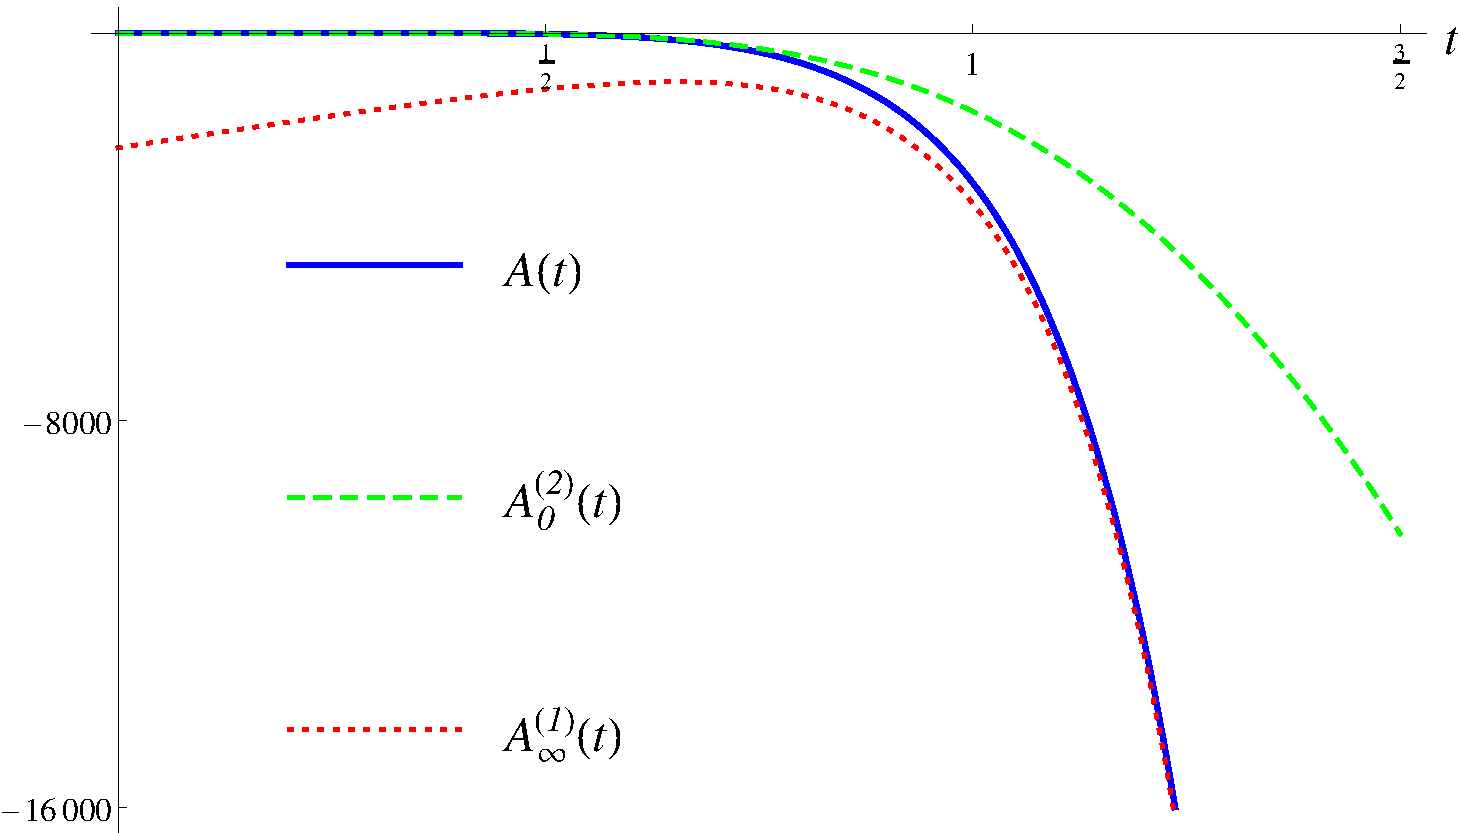
\includegraphics[width=300 pt]{graphics/e8plot_A.pdf}
% \end{figure}

% \noindent We observe that we can compute the values of $A(t)$ for $t\in(0,\infty)$ with any given precision. Indeed, from identities \eqref{eqn: phi0 transform} and \eqref{eqn: psi S define} we obtain the following two presentations for $A(t)$
% \begin{align}
%   A(t)=&-t^2\phi_0(i/t)+\frac{36}{\pi^2}\,t^2\,\psi_S(i/t)\notag\\
%   A(t)=&-t^2\phi_0(it)+\frac{12}{\pi}\,t\,\phi_{-2}(it)-\frac{36}{\pi^2}\,\phi_{-4}(it)-\frac{36}{\pi^2}\,\psi_I(i/t).\notag
% \end{align}
% For an integer $n\geq0$ let $A_0^{(n)}$ and  $A_{\infty}^{(n)}$ be the functions such that
% \begin{align}
%   A(t)=&A_0^{(n)}(t)+O(t^2\,e^{-\pi n /t})\quad\mbox{as}\;t\to0\label{eqn: A asymptotic expansion 0}\\
%   A(t)=&A_\infty^{(n)}(t)+O(t^2\,e^{-\pi n t})\quad\mbox{as}\;t\to\infty.\label{eqn: A asymptotic expansion infty}
% \end{align}
% For each $n\geq 0$ we can compute these functions from the Fourier expansions \eqref{eqn: phi fourier4}--\eqref{eqn: phi fourier0}, \eqref{eqn: psi fourier I}, and \eqref{eqn: psi fourier S}.
%   For example, from \eqref{eqn: phi fourier4}--\eqref{eqn: phi fourier0} and \eqref{eqn: psi fourier I} we compute
% %$$A_\infty^{(0)}(t)=-\frac{72}{\pi^2}\,e^{2\pi t}$$ and
% \begin{align}A_\infty^{(6)}(t)=&\scriptstyle-\tfrac{72}{\pi ^2}\, e^{2 \pi  t}-\tfrac{23328}{\pi ^2}+\tfrac{184320}{\pi ^2}\, e^{-\pi  t}-\tfrac{5194368}{\pi ^2}\, e^{-2 \pi  t}+\tfrac{22560768}{\pi ^2}\, e^{-3 \pi  t}-\tfrac{250583040}{\pi
%     ^2}\, e^{-4 \pi  t}+\tfrac{869916672 }{\pi ^2}\,e^{-5 \pi  t}\notag\\&\scriptstyle+t(\tfrac{8640}{\pi }+\tfrac{2436480}{\pi }\, e^{-2 \pi  t}+\tfrac{113011200 }{\pi }\,e^{-4 \pi  t})-t^2(518400\,e^{-2 \pi  t}+31104000\,e^{-4 \pi  t}).\notag
% \end{align}
% From \eqref{eqn: phi fourier4}--\eqref{eqn: phi fourier0} and \eqref{eqn: psi fourier S} we compute
% %$$A_0^{(2)}(t)=-\frac{368640}{\pi^2}\,t^2\,e^{-\pi /t}$$and
% $$A_0^{(6)}(t)=t^2(-\tfrac{368640}{\pi ^2}\, e^{-\pi/t}-518400\, e^{-2\pi/t}-\tfrac{45121536}{\pi ^2}\, e^{-3\pi/t}-31104000\,e^{-4\pi/t}-\tfrac{1739833344}{\pi ^2}\, e^{-5\pi/t}).$$
% Moreover, from the convergent asymptotic expansion for the Fourier coefficients of a weakly holomorphic modular form \cite[Proposition 1.12]{Bruinier} we find that the $n$-th Fourier coefficient $c_{\psi_I}(n)$ of $\psi_I$ satisfies
% \begin{equation}\label{eqn: Fourier estimate 1}|c_{\psi_I}(n)|\leq e^{4\pi\sqrt{n}}\qquad n\in\tfrac 12 \Z_{>0}.\end{equation} Similar inequalities hold for the Fourier coefficients of $\psi_S$, $\phi_0$, $\phi_{-2}$, and $\phi_{-4}$:
% \begin{align}\label{eqn: Fourier estimate 2}
% &|c_{\psi_S}(n)|\leq 2e^{4\pi\sqrt{n}}\qquad n\in\tfrac 12 \Z_{>0} \\
% &|c_{\phi_0}(n)|\leq 2e^{4\pi\sqrt{n}}\qquad n\in \Z_{>0} \\
% &|c_{\phi_{-2}}(n)|\leq e^{4\pi\sqrt{n}}\qquad n\in  \Z_{>0} \\
% &|c_{\phi_{-4}}(n)|\leq e^{4\pi\sqrt{n}}\qquad n\in \Z_{>0}. \label{eqn: Fourier estimate 5}
%   \end{align}
% Therefore, we can estimate the error terms in the asymptotic expansions \eqref{eqn: A asymptotic expansion 0} and \eqref{eqn: A asymptotic expansion infty} of $A(t)$
% \begin{align}
% \left|A(t)-A_0^{(m)}(t)\right|\leq& (t^2+\frac{36}{\pi^2})\,\sum_{n=m}^\infty 2e^{2\sqrt{2}\pi\sqrt{n}}\,e^{-\pi n/t}\notag\\
% \left|A(t)-A_\infty^{(m)}(t)\right|\leq& (t^2+\frac{12}{\pi}\,t+\frac{36}{\pi^2})\,\sum_{n=m}^\infty 2e^{2\sqrt{2}\pi\sqrt{n}}\,e^{-\pi nt}.\notag
% \end{align}
% For an integer $m\geq0$ we set
% \begin{align}
% R^{(m)}_0:=&(t^2+\frac{36}{\pi^2})\,\sum_{n=m}^\infty 2e^{2\sqrt{2}\pi\sqrt{n}}\,e^{-\pi n/t}\notag\\
% R^{(m)}_\infty:=&(t^2+\frac{12}{\pi}\,t+\frac{36}{\pi^2})\,\sum_{n=m}^\infty 2e^{2\sqrt{2}\pi\sqrt{n}}\,e^{-\pi nt}.\notag
% \end{align}
% Using interval arithmetic we check that
% \begin{align}
% &\left|R_0^{(6)}(t)\right|\leq\left|A_0^{(6)}(t)\right|\quad\mbox{ for }\;t\in(0,1]\notag\\
% &\left|R_\infty^{(6)}(t)\right|\leq\left|A_\infty^{(6)}(t)\right|\quad\mbox{ for }\;t\in[1,\infty)\notag\\
% &A_0^{(6)}(t)<0\quad\mbox{ for }\;t\in(0,1]\notag\\
% &A_\infty^{(6)}(t)<0\quad\mbox{ for }\;t\in[1,\infty).\notag
% \end{align}
% Thus, we see that $A(t)<0$ for $t\in (0,\infty)$. This finishes the proof of the Proposition.
% \end{proof}


% \noindent\textbf{Remark} \emph{Below is the proof from \cite{Via2017}. Similarly to the previous proposition, another (hopefully easier for the formalization) proof of this inequality is given in \cite{Romik2023}}.
% \begin{proof}

% The function $B$ can be also written as
% \begin{align}
%   B(t)=&-t^2\phi_0(i/t)-\frac{36}{\pi^2}\,t^2\,\psi_S(i/t)\notag\\
%   B(t)=&-t^2\phi_0(it)+\frac{12}{\pi}\,t\,\phi_{-2}(it)-\frac{36}{\pi^2}\,\phi_{-4}(it)+\frac{36}{\pi^2}\,\psi_I(i/t).\notag
% \end{align}
% Our aim is to prove that $B(t)>0$ for $t\in(0,\infty)$. A plot of $B(t)$ is given in Figure~\ref{fig:B}.
% \begin{figure}[h!]
% \caption{Plot of the functions $B(t)$, $B^{(2)}_0(t)=\frac{368640}{\pi^2}\,t^2\,e^{-\pi /t}$, and $B^{(1)}_\infty(t)=\frac{8640}{\pi}t-\frac{23328}{\pi^2}$.\label{fig:B}}
%   \centering
% 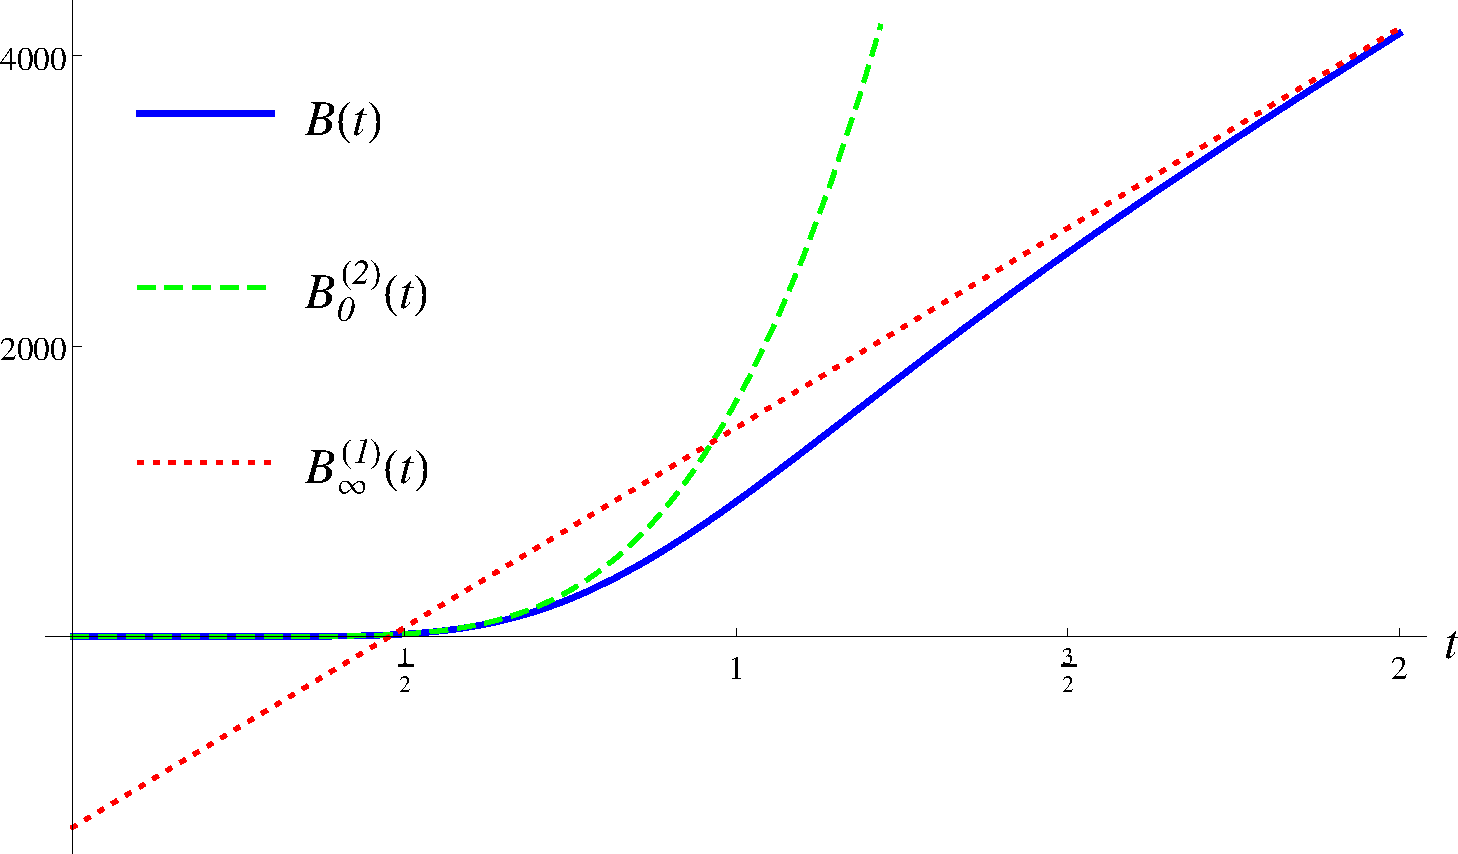
\includegraphics[width=300 pt]{graphics/e8plot_B.pdf}
% \end{figure}

% \noindent For $n\geq 0$ let $B_0^{(n)}$ and  $B_{\infty}^{(n)}$ be the functions  such that
% \begin{align}
%   B(t)=&B_0^{(n)}(t)+O(t^2\,e^{-\pi n /t})\quad\mbox{as}\;t\to0\notag\\
%   B(t)=&B_\infty^{(n)}(t)+O(t^2\,e^{-\pi n t})\quad\mbox{as}\;t\to\infty.\notag
% \end{align}
% We find
% \begin{align}B_\infty^{(6)}(t)=&-\tfrac{12960}{\pi ^2}-\tfrac{184320}{\pi ^2}\,\scriptstyle e^{-\pi  t}\displaystyle-\tfrac{116640}{\pi ^2} \,\scriptstyle e^{-2\pi  t}\displaystyle-\tfrac{22560768}{\pi ^2}\,\scriptstyle e^{-3\pi  t}\displaystyle+\tfrac{56540160}{\pi ^2}\,\scriptstyle e^{-4\pi  t}\displaystyle-\tfrac{869916672 }{\pi ^2} \,\scriptstyle e^{-5\pi  t}\displaystyle\notag\\
% &+t(\tfrac{8640 }{\pi }+\tfrac{2436480}{\pi }\,\scriptstyle e^{-2\pi  t}\displaystyle+\tfrac{113011200 }{\pi }\,\scriptstyle e^{-4\pi  t}\textstyle)-t^2(\scriptstyle518400\,\scriptstyle e^{-2\pi  t}\displaystyle+\scriptstyle31104000\,\scriptstyle e^{-4\pi  t}\displaystyle)\notag
% \end{align}
% and
% $$B_0^{(6)}(t)= t^2(\tfrac{368640}{\pi ^2}\, e^{-\pi/t}-518400\, e^{-2 \pi /t}+\tfrac{45121536 }{\pi ^2}\,e^{-3 \pi/t}-31104000\, e^{-4 \pi/t}+\tfrac{1739833344 }{\pi ^2}\,e^{-5 \pi/t}) .$$
% The estimates \eqref{eqn: Fourier estimate 1}--\eqref{eqn: Fourier estimate 5} imply that $$\left|B(t)-B_0^{(6)}(t)\right|\leq R_0^{(6)}(t)\quad\mbox{for}\;t\in(0,1]$$
% and
% $$\left|B(t)-B_\infty^{(6)}(t)\right|\leq R_\infty^{(6)}(t)\quad\mbox{for}\;t\in[1,\infty).$$
% Using interval arithmetic we verify that
% \begin{align}
% &\left|R_0^{(6)}(t)\right|\leq\left|B_0^{(6)}(t)\right|\quad\mbox{ for }\;t\in(0,1]\notag \\
% &\left|R_\infty^{(6)}(t)\right|\leq\left|B_\infty^{(6)}(t)\right|\quad\mbox{ for }\;t\in[1,\infty)\notag \\
% &B_0^{(6)}(t)>0\quad\mbox{ for }\;t\in(0,1]\notag \\
% &B_\infty^{(6)}(t)>0\quad\mbox{ for }\;t\in[1,\infty). \notag
% \end{align}
% Now identity \eqref{eqn:g B} implies \eqref{eqn:g2}.
% \end{proof}
Finally, we are ready to prove Theorem~\ref{thm:g}.
\begin{theorem}\label{thm:g1}
\uses{prop: a(r) double zeroes, prop: b(r) double zeroes, prop:ineqA, prop:ineqB}
The function
$$g(x):=\frac{\pi\,i}{8640}a(x)+\frac{i}{240\pi}\,b(x)$$
satisfies conditions \eqref{eqn:g1}--\eqref{eqn:g3}.
\end{theorem}
\begin{proof}
First, we prove that \eqref{eqn:g1} holds. By Propositions~\ref{prop: a(r) double zeroes} and \ref{prop: b(r) double zeroes} we know that for $r>\sqrt{2}$
\begin{equation}\label{eqn:g A} g(r)=\frac{\pi}{2160}\,\sin(\pi r^2/2)^2\,\int\limits_0^\infty A(t)\,e^{-\pi r^2 t}\,dt\end{equation}
where $$A(t)=-t^2\phi_0(i/t)-\frac{36}{\pi^2}\,\psi_I(it).$$
from the Proposition~\ref{prop:ineqA} we know that $A(t)<0\quad\mbox{for}\;t\in(0,\infty).$
Therefore identity \eqref{eqn:g A} implies \eqref{eqn:g1}.

Next, we prove \eqref{eqn:g2}. By Propositions~\ref{prop: a another integral} and~\ref{prop: b another integral} we know that for $r>0$
\begin{equation}\label{eqn:g B} \widehat{g}(r)=\frac{\pi}{2160}\,\sin(\pi r^2/2)^2\,\int\limits_0^\infty B(t)\,e^{-\pi r^2 t}\,dt\end{equation}
where $$B(t)=-t^2\phi_0(i/t)+\frac{36}{\pi^2}\,\psi_I(it).$$


Finally, the property \eqref{eqn:g3} readily follows from Proposition~\ref{prop: a values} and Proposition~\ref{prop: b values}.
This finishes the proof of Theorems~\ref{thm:g1} and~\ref{thm:g}.
\end{proof}


\begin{thebibliography}{20}
\bibitem{Abramowitz} {\sc M. Abramowitz, I. Stegun}, \emph{ Handbook of Mathematical Functions with Formulas, Graphs, and Mathematical Tables}, Applied Mathematics Series 55 (10 ed.), New York, USA: United States Department of Commerce, National Bureau of Standards; Dover Publications, 1964.

%\bibitem{BRV} {\sc A. Bondarenko, D. Radchenko, M. Viazovska}, \emph{On optimal asymptotic bounds for spherical designs}, Annals of Math. 178 (2)(2013), pp. 443--452.

\bibitem{Bruinier} {\sc J. Bruinier}, \emph{Borcherds products on O(2,l) and Chern classes of Heegner divisors}, Springer Lecture Notes in Mathematics 1780 (2002)

\bibitem{ElkiesCohn}  {\sc H. Cohn, N. Elkies}, \emph{New upper bounds on sphere packings I}, Annals of Math. 157 (2003) pp. 689--714.

%\bibitem{Cohn} {\sc H. Cohn}, \emph{New upper bounds on sphere packings. II.} Geom. Topol. 6 (2002), pp. 329--353.

%\bibitem{CohnKumar} {\sc H. Cohn, A. Kumar}, \emph{Universally optimal distribution of points on spheres}, J. Amer. Math. Soc. 20 (1) (2007), pp. 99--148.

%\bibitem{ConwaySloan}  {\sc J. H. Conway and N. J. A. Sloane}, \emph{What Are All the Best Sphere Packings in Low Dimensions? ,} Discrete Comput. Geom. (Laszlo Fejes Toth Festschrift), 13 (1995), pp. 383--403.


%\bibitem{DukeImamogluToth} {\sc W. Duke, O. Imamoglu and A. Toth}, {\em Cycle integrals of the j-function and mock modular forms}, Ann. of Math. (2) 173 (2011), no. 2, 947-981.

%\bibitem{Deligne1} {\sc P. Deligne}, \emph{Travaux de Shimura.} S\'eminaire Bourbaki, 23\'eme ann\'ee (1970/71), Exp. No. 389, pp. 123-165. Lecture Notes in Math., Vol. 244, Springer, Berlin, 1971.

%\bibitem{Deligne2} {\sc P. Deligne}, \emph{Vari\'et\'es de Shimura: interpr\'etation modulaire, et techniques de construction de mod\'eles canoniques}, in Automorphic forms, representations and L-functions, Proc. Sympos. Pure Math., XXXIII (Corvallis, OR, 1977), Part 2, pp. 247-289, Amer. Math. Soc., Providence, R.I., 1979.

%\bibitem{CohnZ} {\sc H. Cohn, Y. Zhao}, \emph{Sphere packing bounds via spherical codes}, arXiv:1212.5966 [math.MG]

%\bibitem{Delsarte72} {\sc P. Delsarte},\emph{Bounds for unrestricted codes, by linear programming}, Philips Res. Rep. 27 (1972), pp. 272--289.


%\bibitem{Delsarte77} {\sc P. Delsarte, J. M. Goethals, and J. J. Seidel}, \emph{Spherical codes and designs}, Geom. Dedicata, 6 (1977), pp. 363--388.

\bibitem{first course} {\sc F. Diamond, J. Shurman}, \emph{A First Course in Modular Forms}, Springer New York, 2005.

%\bibitem{Toth} {\sc L. Fejes Toth}, {\em {\"U}ber die dichteste Kugellagerung}, Math. Z. 48 (1943), pp. 676--684.

%\bibitem{Hales} {\sc T. Hales}, {\em A proof of the Kepler conjecture}, Annals of Math. 162 (3) (2005), pp. 1065--1185.

\bibitem{Hejhal} {\sc D. Hejhal}, {\em The Selberg trace formula for $\mathrm{PSL}(2, \R)$},  Springer Lecture Notes in Mathematics 1001 (1983)

%\bibitem{KabLev} {\sc G. A. Kabatiansky and V. I. Levenshtein}, {\em Bounds for packings on a sphere and in space},Problems of Information Transmission 14 (1978), pp. 1--17.

\bibitem{Kohnen} {\sc W. Kohnen}, {\em A Very Simple Proof of the $q$-Product Expansion of the $\Delta$-Function}, The Ramanujan Journal 10 (2005): 71-73.

\bibitem{Lee} {\sc S. Lee}, {\em Algebraic proof of modular form inequalities for optimal sphere packings}, arXiv preprint arXiv:2406.14659 (2024).

\bibitem{Mumford} {\sc D. Mumford}, {\em Tata Lectures on Theta I}, Birkh\"auser, 1983.

%\bibitem{Ma} {\sc Manin, Yu. I.}, {\em Real multiplication and noncommutative geometry (ein Alterstraum)}. The legacy of Niels Henrik Abel, 685-727, Springer, Berlin, 2004.

%\bibitem{MaOdSl} {\sc C. L. Mallows, A. M. Odlyzko, and N. J. A. Sloane}, {\em Upper bounds for modular forms, lattices, and codes}, J. Algebra, 36 (1975), 68--76

\bibitem{Petersson32} {\sc H. Petersson}, {\em Ueber die Entwicklungskoeffizienten der automorphen Formen}, Acta Mathematica, Bd. 58 (1932),  pp. 169--215.

%\bibitem{PfenderZiegler} {\sc F. Pfender, G. M. Ziegler,} {\em Kissing numbers, sphere packings, and some unexpected proofs}, Notice of the AMS  51 (8) (2004) pp. 873--883

\bibitem{Rademacher38} {\sc H. Rademacher and H. S. Zuckerman}, {\em On the Fourier coefficients of certain modular forms of
positive dimension}, Annals of Math. (2) 39 (1938),  pp. 433--462.

\bibitem{Serre73} {\sc J. Serre}, {\em A Course in Arithmetic}, Springer New York, 1973.

%\bibitem{Thue} {\sc A. Thue}, {\em {\"U}ber die dichteste Zusammenstellung von kongruenten Kreisen in einer Ebene}, Norske Vid. Selsk. Skr. No.1 (1910), pp. 1--9.

%\bibitem{Venk}   {\sc  A. Venkatesh}, {\em A Note on Sphere Packings in High Dimension}, International Mathematics Research Notices  7 (2013),  1628--1642

%\bibitem{Yudin} {\sc V. A. Yudin}, {\em Lower bounds for spherical designs}, Izv. Ross. Akad. Nauk. Ser. Mat. 61 (1997), pp. 211-233. English transl., Izv. Math. 6 (1997), pp. 673--683.
% \bibitem{Romik2023} {\sc Dan Romik} {\em On Viazovska’s modular form inequalities} Proceedings of the National Academy of Sciences (USA) 120 (2023), article e2304891120

\bibitem{Via2017} {\sc Maryna S. Viazovska}, {\em The sphere packing problem in dimension 8	},
Pages 991--1015 from Volume 185 (2017), Issue 3.

\bibitem{1-2-3} {\sc D. Zagier}, {\em Elliptic Modular Forms and Their Applications}, In:  The 1-2-3 of Modular Forms, (K. Ranestad, ed.) Norway, Springer Universitext, 2008.
\end{thebibliography}

\newpage

{\footnotesize
\noindent
Ecole Polytechnique Federale de Lausanne\\
1015 Lausanne\\
Switzerland\\
{\it Email address: maryna.viazovska@epfl.ch}}
